% interacttfssample.tex
% v1.05 - August 2017

\documentclass[]{interact}

\usepackage{epstopdf}% To incorporate .eps illustrations using PDFLaTeX, etc.
\usepackage[caption=false]{subfig}% Support for small, `sub' figures and tables
%\usepackage[nolists,tablesfirst]{endfloat}% To `separate' figures and tables from text if required

%\usepackage[doublespacing]{setspace}% To produce a `double spaced' document if required
%\setlength\parindent{24pt}% To increase paragraph indentation when line spacing is doubled
%\setlength\bibindent{2em}% To increase hanging indent in bibliography when line spacing is doubled

\usepackage[numbers,sort&compress]{natbib}% Citation support using natbib.sty
\bibpunct[, ]{[}{]}{,}{n}{,}{,}% Citation support using natbib.sty
\renewcommand\bibfont{\fontsize{10}{12}\selectfont}% Bibliography support using natbib.sty

\theoremstyle{plain}% Theorem-like structures provided by amsthm.sty
\newtheorem{theorem}{Theorem}[section]
\newtheorem{lemma}[theorem]{Lemma}
\newtheorem{corollary}[theorem]{Corollary}
\newtheorem{proposition}[theorem]{Proposition}

\theoremstyle{definition}
\newtheorem{definition}[theorem]{Definition}
\newtheorem{example}[theorem]{Example}

\theoremstyle{remark}
\newtheorem{remark}{Remark}
\newtheorem{notation}{Notation}

\allowdisplaybreaks
\usepackage{hyperref}
\usepackage{mathtools}
\usepackage{float}
\renewcommand{\ln}[1]{\ensuremath{\text{ln}\abs{#1}}}
\newcommand{\abs}[1]{\ensuremath{\left| #1 \right|}}
\renewcommand{\exp}[1]{\ensuremath{\text{exp}\left( #1 \right)}}
\newcommand{\diff}[3][]{
    \ifthenelse
    {\equal{#1}{}}
    {\ensuremath{\frac{\opdiff{#2}}{\opdiff{#3}}}}
    {\ensuremath{\frac{\mathrm{d}^{#1}#2}{\mathrm{d}#3^{#1}}}}
    }
\newcommand{\opdiff}[1]{\ensuremath{\mathrm{d}#1}}
\newcommand{\myref}[2][]{%
    \ifthenelse{\equal{#1}{Equation} \OR \equal{#1}{System} \OR \equal{#1}{Model} \OR \equal{#1}{Matrix} \OR \equal{#1}{Theorem} \OR \equal{#1}{Parameters} \OR \equal{#1}{parameters}}
    {#1~\eqref{#2}}
    {#1~\ref{#2}}%
}
\graphicspath{{figures/eps/}}
\numberwithin{equation}{section}

\begin{document}

\articletype{}% Specify the article type or omit as appropriate

\title{Complex Dynamics of a Three Species Ecosystem}

\author{
\name{Ramsey "Rayla" Phuc\textsuperscript{a} and Ephraim Agyingi\textsuperscript{a}}
\affil{\textsuperscript{a}Department of Mathematics and Statistics, Rochester Institute of Technology, USA}
}

\maketitle

% Z: Chimps
% Y: Smaller monkeys
% X: 

\begin{abstract}
This paper investigates the dynamics of an ecological system of three species with three different interactions, those being mutualism, amensalism, and non-linear competition. We determine the equilibrium points and conduct a comprehensive analysis of their characteristics. Numerical computations are performed to assess the stability or instability of the newly derived equilibrium points. The obtained results offer valuable insights into the dynamics and stability of the modified model, shedding light on the consequences of mutualism and amensalism interactions in the examined ecological system. This research contributes to a deeper understanding of the interrelationships between species interactions and population dynamics in ecological systems.
\end{abstract}

\begin{keywords}
Mutualism; Amensalism; Non-Linear Competition; Holling-Type II Response; Refuge; Hopf Bifurcation
\end{keywords}


% ----------------------------------------------------------------------------
% Author: Rayla Kurosaki
% GitHub: https://github.com/rkp1503
% ----------------------------------------------------------------------------

\section{Introduction}\label{sec:introduction}
In the vast realm of biological sciences, understanding the complex interplay of various phenomena is a formidable challenge. Nature's intricacies often defy direct observation and experimentation, necessitating the development of powerful tools that can unravel its hidden patterns. Enter mathematical models, a transformative approach that harnesses the language of mathematics to dissect, analyze, and predict the behavior of biological systems. These models serve as indispensable bridges between theoretical abstractions and empirical realities, enabling scientists to gain deeper insights into the fundamental principles that govern living organisms. By quantifying and formalizing biological processes, mathematical models offer a systematic framework to study intricate dynamics, investigate the consequences of different hypotheses, and guide experimental design.

There have been a plethora of models created to analyze the dynamics of such ecosystems. There are models which considers two species~\cite{GHOSH2017110, CHEN20122790, YU2012208167, HUANG2006672, AZIZALAOUI20031069, XIAO200614, SEN201212, CANTRELL2001206, CHEN20092905, CHEN2010246, KAR2005681, CHATTOPADHYAY1996287, KAR2003125}, three species~\cite{GAKKHAR201654, PANJA2022100153, MENG2014810, ALIDOUSTI2020109688, PEET2005491, SARWARDI2012133, PRIYADARSHI20133202, GAKKHAR2005105, GAKKHAR2007808, Mukherjee2013, DHAKNEMUNDE2012, CHATTOPADHYAY200345, PANJAMONDAL2015, PANJA2017389, KHAJANCHI2017193, JANA2017350} and four species~\cite{JANA2021100942}. Some of these models incorporate a functional response in their model, which include the Beddington–DeAngelis functional response~\cite{CANTRELL2001206}, the Crowley–Martin type functional response~\cite{MENG2014810}, the Holling-type I functional response~\cite{JANA2021100942, Mukherjee2013, CHATTOPADHYAY200345}, the Holling-type II functional response~\cite{GAKKHAR201654, PANJA2022100153, JANA2021100942, GHOSH2017110, YU2012208167, HUANG2006672, AZIZALAOUI20031069, CHEN2010246, SARWARDI2012133, PRIYADARSHI20133202, GAKKHAR2005105, GAKKHAR2007808, Mukherjee2013, CHATTOPADHYAY200345, PANJAMONDAL2015, JANA2017350}, the Holling-type III functional response~\cite{CHATTOPADHYAY200345}, the Leslie-Gower functional response~\cite{YU2012208167, AZIZALAOUI20031069, PRIYADARSHI20133202}, the Monod-Haldane type functional response~\cite{ALIDOUSTI2020109688}, and the Ratio-dependent functional response~\cite{XIAO200614, SEN201212, CANTRELL2001206, KHAJANCHI2017193}. Some models consider prey refuge~\cite{GAKKHAR201654, PANJA2022100153, GHOSH2017110, CHEN20122790, HUANG2006672, CHEN20092905, CHEN2010246, KAR2005681, SARWARDI2012133, Mukherjee2013, KHAJANCHI2017193, JANA2017350}, harvesting~\cite{XIAO200614, KAR2003125, PANJA2017389}, and the Allee effect~\cite{SEN201212}.

In this paper, we will consider a biological system that involves three species with each pairing of species have a unique interaction. In particular, we will study an ecosystem which involves predation, non-linear mutualism, and amensalism. The pairing of species that are in a predation interaction incorporates the Holling type II functional response and refuge into consideration.

% ----------------------------------------------------------------------------
% Author: Ramsey (Rayla) Phuc
% Alias: Rayla Kurosaki
% GitHub: https://github.com/rkp1503
% 
% Co-author: Ephraim Agyingi
% ----------------------------------------------------------------------------
\chapter{Proposed Model}\label{ch:proposed-model}
In this chapter, we will breifly introduce the desired problem to model and make some assumptions. Then we will construct a non-dimensionalized model from the assumptions. Finally, we will show some important properties the model has.

\section{Problem Statement and Assumptions}
Consider an ecosystem which involves three species, $X,\ Y,\ Z$. Species $X,\ Y,\ Z$ grows logistically at their respective intrinsic growth rate $r_x>0,\ r_y>0,\ r_z>0$ with their respective carrying capacity $K_x>0,\ K_y>0,\ K_z>0$ and species $Z$ dies at a rate of $e$. We will also assume that each pairing of species has a unique interaction with one another. In particular, we will model an ecosystem where mutualism, predation, and amensalism are present. % Provide a real life example of this type of interaction if possible.

We will assume that species $X,\ Y$ are in a non-linear mutualism relationship. Members from both species will interact with one another that will help both species in some way. As a result, each species will be affected by one another in some way. To illustrate this, we will let $\alpha_{xy} > 0$ be the inter-species mutualism coefficient where species $X$ is being affected by species $Y$ and $\alpha_{yx} > 0$ be the inter-species mutualism coefficient where species $Y$ is being affected by species $X$.

We will assume that species $Y,\ Z$ are in a predation relationship where species $Z$ preys on species $Y$ with the Holling type II response and with an attack rate of $a$. As a result of this, a proportion $0 \leq p \leq 1$ of species $Y$ will take refuge into species $Z$ with a conservation rate of $c$. 

We will assume that species $X,\ Z$ are in an amensalism relationship where species $X$ is the species being detrimented and species $Z$ will remain unaffected. In this relationship, species $X$ is begin detrimented at a rate of $\delta_{xz} \geq 0$, which we will call the amensalism coefficient. 

\section{Building the Model of this Ecosystem}\label{sec:building-the-model-of-this-ecosystem}
With these assumptions, the governing system of equations that accurately describes this type of ecosystem are:
\begin{subequations}\label{model:rayla-ephraim-d}
    \begin{align}
        \diff[]{X}{T} &= r_xX\left(1-\frac{X}{K_x}+\frac{\alpha_{xy}Y^2}{K_x}\right)-\delta_{xz}XZ
        \label{eq:rayla-ephraim-d-x}\\
        \diff[]{Y}{T} &= r_yY\left(1-\frac{Y}{K_y}+\frac{\alpha_{yx}X^2}{K_y}\right)-\frac{a\left(1-p\right)YZ}{b+\left(1-p\right)Y}
        \label{eq:rayla-ephraim-d-y}\\
        \diff[]{Z}{T} &= r_zZ\left(1-\frac{Z}{K_z}\right)+Z\left(\frac{ac\left(1-p\right)Y}{b+\left(1-p\right)Y}-e\right)
        \label{eq:rayla-ephraim-d-z}
    \end{align}
\end{subequations}

with the initial conditions $X(0) \geq 0,\ Y(0) \geq 0,\ Z(0) \geq 0$. Then using the following substitutions:

\begin{gather*}
    X=K_xx,\ Y=K_yy,\ Z=K_zz,\ T=\frac{1}{r_x}t,\ r_{yx}=\frac{r_y}{r_x},\ r_{zx}=\frac{r_z}{r_x}\\
    \varphi_{xy}=\frac{\alpha_{xy}K_y^2}{K_x},\ \varphi_{yx}=\frac{\alpha_{yx}K_x^2}{K_y},\ \varphi_{xz}=\frac{\delta_{xz}K_z}{r_x},\ u_1=\frac{aK_z}{r_xK_y},\ u_2=\frac{b}{K_y},\ u_3=\frac{ac}{r_x},\ u_4=\frac{e}{r_x}
\end{gather*}

we can simplify and non-dimensionalize \myref[Model]{model:rayla-ephraim-d}. This gives us the following model we will work on throughout this paper:
\begin{subequations}\label{model:rayla-ephraim}
    \begin{align}
        \diff[]{x}{t} &= x\left(1-x+\varphi_{xy}y^2\right)-\varphi_{xz}xz
        \label{eq:rayla-ephraim-x}\\
        \diff[]{y}{t} &= r_{yx}y\left(1-y+\varphi_{yx}x^2\right)-\frac{u_1\left(1-p\right)yz}{u_2+\left(1-p\right)y}
        \label{eq:rayla-ephraim-y}\\
        \diff[]{z}{t} &= r_{zx}z\left(1-z\right)+z\left(\frac{u_3\left(1-p\right)y}{u_2+\left(1-p\right)y}-u_4\right)
        \label{eq:rayla-ephraim-z}
    \end{align}
\end{subequations}

with the initial conditions $x(0) \geq 0,\ y(0) \geq 0,\ z(0) \geq 0$.

\section{Unique properties of the Proposed Model}
When creating a model that encapsulates an ecosystem, we need to make sure that it makes sense. In biology, a negative population does not make sense. To show that \myref[Model]{model:rayla-ephraim} makes sense, we will need to show that for any non-negative starting populations, \myref[Model]{model:rayla-ephraim} will provide a non-negative solution. This is shown in \myref[Theorem]{thm:positiveness}.

\begin{theorem}\label{thm:positiveness}
    For any set of intiial conditions $x(0) = x_0,\ y(0) = y_0,\ z(0) = z_0$ where $x_0 > 0,\ y_0 > 0,\ z_0 > 0$, \myref[Model]{model:rayla-ephraim} only has non-negative solutions.
\end{theorem}
\begin{proof}
    Starting with \myref[Equation]{eq:rayla-ephraim-x}, we can factor out an $x$:
    \begin{equation*}
        \diff[]{x}{t} = x\left(1-x+\varphi_{xy}y^2-\varphi_{xz}z\right)
    \end{equation*}
    From here, we can perform separation of variables:
    \begin{equation*}
        \frac{1}{x}\ \opdiff{x} = \left(1-x+\varphi_{xy}y^2-\varphi_{xz}z\right)\ \opdiff{t}
    \end{equation*}
    We can then integrate both sides from $t=0$ to $t=\tau$ for some time $\tau>0$:
    \begin{equation*}
        \int_0^\tau \frac{1}{x}\ \opdiff{x} = \int_0^\tau \left(1-x+\varphi_{xy}y^2-\varphi_{xz}z\right)\ \opdiff{t}
    \end{equation*}
    The left hand side evaluates to:
    \begin{equation*}
        \ln{x(\tau)}-\ln{x(0)} = \int_0^\tau \left(1-x+\varphi_{xy}y^2-\varphi_{xz}z\right)\ \opdiff{t}
    \end{equation*}
    Solving for $x(\tau)$ yields:
    \begin{equation*}
        x(\tau) = x(0)\ \exp{\int_0^\tau \left(1-x+\varphi_{xy}y^2-\varphi_{xz}z\right)\ \opdiff{t}}
    \end{equation*}
    Note that on the right hand side, we have an exponential function. Since $x(0) > 0$, this means that will never be negative. Thus, we can conclude that $x(\tau) \geq 0$. From \myref[Equation]{eq:rayla-ephraim-y}, we can factor out an $y$:
    \begin{equation*}
        \diff[]{y}{t} = y\left(r_{yx}\left(1-y+\varphi_{yx}x^2\right)-\frac{u_1\left(1-p\right)z}{u_2+\left(1-p\right)y}\right)
    \end{equation*}
    From here, we can perform separation of variables:
    \begin{equation*}
        \frac{1}{y}\ \opdiff{y} = \left(r_{yx}\left(1-y+\varphi_{yx}x^2\right)-\frac{u_1\left(1-p\right)z}{u_2+\left(1-p\right)y}\right)\ \opdiff{t}
    \end{equation*}
    We can then integrate both sides from 0 to $\tau$:
    \begin{equation*}
        \int_0^\tau \frac{1}{y}\ \opdiff{y} = \int_0^\tau \left(r_{yx}\left(1-y+\varphi_{yx}x^2\right)-\frac{u_1\left(1-p\right)z}{u_2+\left(1-p\right)y}\right)\ \opdiff{t}
    \end{equation*}
    The left hand side evaluates to:
    \begin{equation*}
        \ln{y(\tau)}-\ln{y(0)} = \int_0^\tau \left(r_{yx}\left(1-y+\varphi_{yx}x^2\right)-\frac{u_1\left(1-p\right)z}{u_2+\left(1-p\right)y}\right)\ \opdiff{t}
    \end{equation*}
    Solving for $x(\tau)$ yields:
    \begin{equation*}
        y(\tau) = y(0)\ \exp{\int_0^\tau \left(r_{yx}\left(1-y+\varphi_{yx}x^2\right)-\frac{u_1\left(1-p\right)z}{u_2+\left(1-p\right)y}\right)\ \opdiff{t}}
    \end{equation*}
    Note that on the right hand side, we have an exponential function. Since $y(0) > 0$, this means that will never be negative. Thus, we can conclude that $y(\tau) \geq 0$. From \myref[Equation]{eq:rayla-ephraim-z}, we can factor out an $z$:
    \begin{equation*}
        \diff[]{z}{t} = z\left(r_{zx}\left(1-z\right)+\left(\frac{u_3\left(1-p\right)y}{u_2+\left(1-p\right)y}-u_4\right)\right)
    \end{equation*}
    From here, we can perform separation of variables:
    \begin{equation*}
        \frac{1}{z}\ \opdiff{z} = \left(r_{zx}\left(1-z\right)+\left(\frac{u_3\left(1-p\right)y}{u_2+\left(1-p\right)y}-u_4\right)\right)\ \opdiff{t}
    \end{equation*}
    We can then integrate both sides from 0 to $\tau$:
    \begin{equation*}
        \int_0^\tau \frac{1}{z}\ \opdiff{z} = \int_0^\tau \left(r_{zx}\left(1-z\right)+\left(\frac{u_3\left(1-p\right)y}{u_2+\left(1-p\right)y}-u_4\right)\right)\ \opdiff{t}
    \end{equation*}
    The left hand side evaluates to:
    \begin{equation*}
        \ln{z(\tau)}-\ln{z(0)} = \int_0^\tau \left(r_{zx}\left(1-z\right)+\left(\frac{u_3\left(1-p\right)y}{u_2+\left(1-p\right)y}-u_4\right)\right)\ \opdiff{t}
    \end{equation*}
    Solving for $x(\tau)$ yields:
    \begin{equation*}
        z(\tau) = z(0)\ \exp{\int_0^\tau \left(r_{zx}\left(1-z\right)+\left(\frac{u_3\left(1-p\right)y}{u_2+\left(1-p\right)y}-u_4\right)\right)\ \opdiff{t}}
    \end{equation*}
    Note that on the right hand side, we have an exponential function. Since $z(0) > 0$, this means that will never be negative. Thus, we can conclude that $z(\tau) \geq 0$. Since we have shown that $x(\tau) \geq 0,\ y(\tau) \geq 0,\ z(\tau) \geq 0$ for some time $\tau > 0$, this implies that \myref[Model]{model:rayla-ephraim} will have non-negative solutions for non-negative initial conditions.
\end{proof}

Even though we have shown that \myref[Model]{model:rayla-ephraim} will always be non-negative for any set of non-negative initial conditions though \myref[Theorem]{thm:positiveness}, that is not enough to show that \myref[Model]{model:rayla-ephraim} makes sense. Populations have not just a lower limit, but also an upper limit. A population cannot just grow infinitely in size. After some time, a population will get to the point where it cannot grow any further. Thus, we will need to show that out model is uniformly boundeded. This is shown in \myref[Theorem]{thm:bounded}.

\begin{theorem}\label{thm:bounded}
    For any set of initial conditions $x(0) = x_0,\ y(0) = y_0,\ z(0) = z_0$ where $x_0 > 0,\ y_0 > 0,\ z_0 > 0$, \myref[Model]{model:rayla-ephraim} is bounded above uniformly.
\end{theorem}
\begin{proof}
    % \begin{align*}
    %     V &= ax^2+by^2+cz^2\\
    %     \diff[]{V}{t} &= 2a\diff[]{x}{t}+2b\diff[]{y}{t}+2c\diff[]{z}{t}\\
    %     \diff[]{V}{t} &= 2a\left(x\left(1-x+\varphi_{xy}y^2\right)-\varphi_{xz}xz\right)\\
    %     & +2b\left(r_{yx}y\left(1-y+\varphi_{yx}x^2\right)-\frac{u_1\left(1-p\right)yz}{u_2+\left(1-p\right)y}\right)\\
    %     & +2c\left(r_{zx}z\left(1-z\right)+z\left(\frac{u_3\left(1-p\right)y}{u_2+\left(1-p\right)y}-u_4\right)\right)\\
    %     \diff[]{V}{t} &= 2ax-2ax^2+2a\varphi_{xy}xy^2-2a\varphi_{xz}xz+2br_{yx}y-2br_{yx}y^2+2br_{yx}\varphi_{yx}x^2y-\frac{2bu_1\left(1-p\right)yz}{u_2+\left(1-p\right)y}+2cr_{zx}z\\
    %     &-2cr_{zx}z^2+\frac{2cu_3\left(1-p\right)yz}{u_2+\left(1-p\right)y}-2cu_4z
    %     % &= 2a\left(x\left(1-x+\varphi_{xy}y^2\right)-\varphi_{xz}xz\right)+2b\left(r_{yx}y\left(1-y+\varphi_{yx}x^2\right)-\frac{u_1\left(1-p\right)yz}{u_2+\left(1-p\right)y}\right)+2c\left(r_{zx}z\left(1-z\right)+z\left(\frac{u_3\left(1-p\right)y}{u_2+\left(1-p\right)y}-u_4\right)\right)
    % \end{align*}
    Here, we will start by placing an upper bound for \myref[Equation]{eq:rayla-ephraim-d-z}:
    \begin{equation*}
        \diff[]{z}{t} \leq r_{zx}z\left(1-z\right)+z\left(u_3-u_4\right)
    \end{equation*}
    From here, we can perform separation of variables:\
    \begin{equation*}
        \frac{1}{z\left(u_3-u_4+r_{zx}-r_{zx}z\right)}\ \opdiff{z} \leq \opdiff{t}
    \end{equation*}
    Interating both sides, we obtain the following inequality:
    \begin{equation*}
        z(t) < \frac{\left(u_3-u_4+r_{zx}\right)z_0}{\exp{\left(u_4-u_3-r_{zx}\right)t}+r_{zx}z_0}
    \end{equation*}
    from which we can conclude that:
    \begin{equation*}
        \lim_{t\to\infty} \frac{\left(u_3-u_4+r_{zx}\right)z_0}{\exp{\left(u_4-u_3-r_{zx}\right)t}+r_{zx}z_0} = 1+\frac{u_3-u_4}{r_{zx}}
    \end{equation*}
    thus proving that $z$ is bounded above uniformly. Now consider the following function:
    \begin{equation*}
        f_1 = y + \frac{u_1}{u_3}z
    \end{equation*}
    The derivative of this function with respect to $t$ is:
    \begin{equation*}
        \diff[]{f_1}{t} = \diff[]{y}{t} + \frac{u_1}{u_3}\diff[]{z}{t}
    \end{equation*}
    \begin{align*}
        \diff[]{f_1}{t} &= \diff[]{y}{t} + \frac{u_1}{u_3}\diff[]{z}{t}\\
        \diff[]{f_1}{t} &= r_{yx}y\left(1-y+\varphi_{yx}x^2\right)-\frac{u_1\left(1-p\right)yz}{u_2+\left(1-p\right)y}+\frac{u_1}{u_3}\left(r_{zx}z\left(1-z\right)+z\left(\frac{u_3\left(1-p\right)y}{u_2+\left(1-p\right)y}-u_4\right)\right)\\
        \diff[]{f_1}{t} &= r_{yx}y\left(1-y+\varphi_{yx}x^2\right)-\frac{u_1\left(1-p\right)yz}{u_2+\left(1-p\right)y}+\frac{r_{zx}u_1z\left(1-z\right)}{u_3}+\frac{u_1\left(1-p\right)yz}{u_2+\left(1-p\right)y}-\frac{u_1u_4z}{u_3}\\
        \diff[]{f_1}{t} &= r_{yx}y\left(1-y+\varphi_{yx}x^2\right)+\frac{r_{zx}u_1}{u_3}z\left(1-z\right)-\frac{u_1u_4z}{u_3}
    \end{align*}
\end{proof}

% ----------------------------------------------------------------------------
% Author: Ramsey (Rayla) Phuc
% Alias: Rayla Kurosaki
% GitHub: https://github.com/rkp1503
% 
% Co-author: Ephraim Agyingi
% ----------------------------------------------------------------------------
\chapter{Equilibria analysis}\label{ch:equilibria-analysis}
In \myref[Chapter]{ch:proposed-model}, we have modified some of the assumptions the previous authors have made to create \myref[Model]{model:rayla-ephraim}. In addition, we have proved that \myref[Model]{model:rayla-ephraim} only has non-negative solutions for any set of non-negative initial conditions via \myref[Theorem]{thm:positiveness}. In this chapter, we will identify, classify, and determine the stability of all the equilibria points that exists in \myref[Model]{model:rayla-ephraim}. 

\section{Identifying Equilibria}
We will start by identifying all the equilibria of \myref[Model]{model:rayla-ephraim}, which is done by setting all the equations equal to 0 and solving for each variable~\cite{Strogatz9780813349107}. Thus, we have to solve for $x^*,\ y^*,\ z^*$ in the following system of equations:

\begin{subequations}\label{system:model-0}
    \begin{align}
        0 &= x^*\left(1-x^*+\varphi_{xy}\left(y^*\right)^2\right)-\varphi_{xz}x^*z^* \label{eq:model-0-x}\\
        0 &= r_{yx}y^*\left(1-y^*+\varphi_{yx}\left(x^*\right)^2\right)-\frac{u_1\left(1-p\right)y^*z^*}{u_2+\left(1-p\right)y^*} \label{eq:model-0-y}\\
        0 &= r_{zx}z^*\left(1-z^*\right)+z^*\left(\frac{u_3\left(1-p\right)y^*}{u_2+\left(1-p\right)y^*}-u_4\right) \label{eq:model-0-z}
    \end{align}
\end{subequations}

\begin{theorem}\label{thm:eq-trivial-exist}
    The trivial equilibrium point $E_0=\left(0,\ 0,\ 0\right)$ always exist.
\end{theorem}
\begin{proof}
    The trivial equilibrium point is an equilibrium point $E=\left(x^*,\ y^*,\ z^*\right)$ where $x^*=y^*=z^*=0$. Plugging in $x^*=0,\ y^*=0,\ z^*=0$ into \myref[System]{system:model-0}, we can see that each equation reduces to $0=0$. Thus, we have proved that the trivial equilibrium point $E_0=\left(0,\ 0,\ 0\right)$ always exist.
\end{proof}

\begin{theorem}\label{thm:eq-axial-x-exist}
    The $x$-axial equilibrium point $E_x=\left(1,\ 0,\ 0\right)$ always exist.
\end{theorem}
\begin{proof}
    The $x$-axial equilibrium point is an equilibrium point $E=\left(x^*,\ y^*,\ z^*\right)$ where $x^*\neq0$ and $y^*=z^*=0$. Since we are dealing with populations, we should not consider values where $x^*<0$. Thus, a more appropriate constraint is $x^*>0$. Plugging in $y^*=0,\ z^*=0$ into \myref[System]{system:model-0}, we can see that both \myref[Equation]{eq:model-0-y} and \myref[Equation]{eq:model-0-z} reduces to $0=0$ while \myref[Equation]{eq:model-0-x} reduces to

    \begin{equation*}
        x^*\left(1-x^*\right)=0
    \end{equation*}

    which has solutions $x^*=\left\{0,1\right\}$. With the constraint $x^*>0$, we have proved that the $x$-axial equilibrium point $E_x=\left(1,\ 0,\ 0\right)$ always exist.
\end{proof}

\begin{theorem}\label{thm:eq-axial-y-exist}
    The $y$-axial equilibrium point $E_y=\left(0,\ 1,\ 0\right)$ always exist.
\end{theorem}
\begin{proof}
    The $y$-axial equilibrium point is an equilibrium point $E=\left(x^*,\ y^*,\ z^*\right)$ where $y^*>0$ and $x^*=z^*=0$. Plugging in $x^*=0,\ z^*=0$ into \myref[System]{system:model-0}, we can see that both \myref[Equation]{eq:model-0-x} and \myref[Equation]{eq:model-0-z} reduces to $0=0$ while \myref[Equation]{eq:model-0-y} reduces to

    \begin{equation*}
        r_{yx}y^*\left(1-y^*\right)=0
    \end{equation*}

    which has solutions $y^*=\left\{0,1\right\}$. With the cosntraint $y^*>0$, we have proved that the $y$-axial equilibrium point $E_y=\left(0,\ 1,\ 0\right)$ always exist.
\end{proof}

\begin{theorem}\label{thm:eq-axial-z-exist}
    The $z$-axial equilibrium point $E_z=\left(0,\ 0,\ z^*\right)$ exist where
    
    \begin{equation*}
        z^* = 1-\frac{u_4}{r_{zx}}
    \end{equation*}

    under the condition where $r_{zx}>u_4$.
\end{theorem}
\begin{proof}
    The $z$-axial equilibrium point is an equilibrium point $E=\left(x^*,\ y^*,\ z^*\right)$ where $z^*>0$ and $x^*=y^*=0$. Plugging in $x^*=0,\ y^*=0$ into \myref[System]{system:model-0}, we can see that both \myref[Equation]{eq:model-0-x} and \myref[Equation]{eq:model-0-y} reduces to $0=0$ while \myref[Equation]{eq:model-0-z} reduces to

    \begin{equation*}
        r_{zx}z^*\left(1-z^*\right)-u_4z^*=0
    \end{equation*}

    which has solutions
    
    \begin{equation*}
        z^*=\left\{0,1-\frac{u_4}{r_{zx}}\right\}
    \end{equation*}
    
    With the cosntraint $z^*>0$, we have proved that the $z$-axial equilibrium point $E_z=\left(0,\ 0,\ z^*\right)$ exist where
    
    \begin{equation*}
        z^* = 1-\frac{u_4}{r_{zx}}
    \end{equation*}

    under the condition where $r_{zx}>u_4$.
\end{proof}

\begin{theorem}\label{thm:eq-boundary-xy-exist}
    The $xy$-boundary equilibrium point $E_{xy}=\left(x^*,\ y^*,\ 0\right)$ exist where $x^*=1+\varphi_{xy}\left(y^*\right)^2$ and $y^*$ is a positive solution to

    \begin{equation*}
        \varphi_{xy}^2\varphi_{yx}\left(y^*\right)^4+2\varphi_{xy}\varphi_{yx}\left(y^*\right)^2-y^*+\varphi_{yx}+1=0
    \end{equation*}

    which can be acheived under the following condition
    
    \begin{equation*}
        \varphi_{yx}<\frac{\beta-1}{\left(\varphi_{xy}\beta^2+1\right)^2}
    \end{equation*}
    
    for some $\beta\in\left(1, \infty\right)$.
\end{theorem}
\begin{proof}
    The $xy$-boundary equilibrium point is an equilibrium point $E=\left(x^*,\ y^*,\ z^*\right)$ where $x^*>0,\ y^*>0$ and $z^*=0$. Plugging in $z^*=0$ into \myref[System]{system:model-0}, we can see that \myref[Equation]{eq:model-0-z} reduces to $0=0$ which leaves us with the following system to solve:

    \begin{subequations}\label{system:xy-boundary}
        \begin{align}
            0 &= 1-x^*+\varphi_{xy}\left(y^*\right)^2 \label{eq:xy-boundary-x}\\
            0 &= 1-y^*+\varphi_{yx}\left(x^*\right)^2 \label{eq:xy-boundary-y}
        \end{align}
    \end{subequations}

    Solving for $x^*$ in \myref[Equation]{eq:xy-boundary-x} we obtain $x^*=1+\varphi_{xy}\left(y^*\right)^2$. We can plug this into \myref[Equation]{eq:xy-boundary-y} to obtain the following equation in terms of $y^*$:

    \begin{equation*}
        \varphi_{xy}^2\varphi_{yx}\left(y^*\right)^4+2\varphi_{xy}\varphi_{yx}\left(y^*\right)^2-y^*+\varphi_{yx}+1=0
    \end{equation*}

    There is no nice, closed-form solution for $y^*$ but it is sufficient to show that a positive solution $y^*>0$ exists. First, lets treat the equation above as a function of $y^*$:

    \begin{equation*}
        f\left(y^*\right)=\varphi_{xy}^2\varphi_{yx}\left(y^*\right)^4+2\varphi_{xy}\varphi_{yx}\left(y^*\right)^2-y^*+\varphi_{yx}+1
    \end{equation*}

    Note that $f\left(y^*\right)$ is continuous for all $y^*>0$ and $f(0)=\varphi_{yx}+1>0$. By the Intermediate Value Theorem~\cite{STEWART9781337613927}, we can say that there exist a value $\beta\in\left(0,\infty\right)$ such that $f(\beta)=0$. Thus, a solution to $f\left(y^*\right)=0$ exists if for some $\beta\in\left(0,\infty\right)$, $f\left(\beta\right)<0$, or:

    \begin{equation}\label{eq:xy-eq-condition}
        \varphi_{yx}<\frac{\beta-1}{\left(\varphi_{xy}\beta^2+1\right)^2}
    \end{equation}

    Note that if $\beta\in(0, 1]$, then the right hand side of \myref[Equation]{eq:xy-eq-condition} will be negative implying that $\varphi_{yx}<0$. However, since all parameters are positive, we cannot have $\beta$ fall in this range. Therefore, we know that $\beta\in\left(1,\infty\right)$. With this, we have proved that the $xy$-boundary equilibrium point $E_{xy}=\left(x^*,\ y^*,\ 0\right)$ exist where $x^*=1+\varphi_{xy}\left(y^*\right)^2$ and $y^*$ is a positive solution to

    \begin{equation*}
        \varphi_{xy}^2\varphi_{yx}\left(y^*\right)^4+2\varphi_{xy}\varphi_{yx}\left(y^*\right)^2-y^*+\varphi_{yx}+1=0
    \end{equation*}

    which can be acheived under the following condition
    
    \begin{equation*}
        \varphi_{yx}<\frac{\beta-1}{\left(\varphi_{xy}\beta^2+1\right)^2}
    \end{equation*}
    
    for some $\beta\in\left(1, \infty\right)$.
\end{proof}

\begin{theorem}\label{thm:eq-boundary-xz-exist}
    The $xz$-boundary equilibrium point $E_{xz}=\left(x^*,\ 0,\ z^*\right)$ exist where 
    
    \begin{equation*}
        x^*=1-\varphi_{xz}\left(1-\frac{u_4}{r_{zx}}\right),\quad z^*=1-\frac{u_4}{r_{zx}}
    \end{equation*}
    
    provided that the conditions
    
    \begin{equation*}
        \varphi_{xz}<\frac{r_{zx}}{r_{zx}-u_4},\quad r_{zx}>u_4
    \end{equation*}
    
    have been satisfied.
\end{theorem}
\begin{proof}
    The $xz$-boundary equilibrium point is an equilibrium point $E=\left(x^*,\ y^*,\ z^*\right)$ where $x^*>0,\ z^*>0$ and $y^*=0$. Plugging in $y^*=0$ into \myref[System]{system:model-0}, we can see that \myref[Equation]{eq:model-0-y} reduces to $0=0$ which leaves us with the following system to solve:

    \begin{subequations}\label{system:xz-boundary}
        \begin{align}
            0 &= 1-x^*-\varphi_{xz}z^* \label{eq:xz-boundary-x}\\
            0 &= r_{zx}\left(1-z^*\right)-u_4 \label{eq:xz-boundary-z}
        \end{align}
    \end{subequations}

    Solving for $z^*$ in \myref[Equation]{eq:xz-boundary-z} we obtain
    
    \begin{equation*}
        z^*=1-\frac{u_4}{r_{zx}}
    \end{equation*}
    
    Here, we know that $z^*>0$ so this solution we found implies $r_{zx}>u_4$. We can plug this solution of $z^*$ into \myref[Equation]{eq:xz-boundary-x} and solve for $x^*$, which yields 
    
    \begin{equation*}
        x^*=1-\varphi_{xz}\left(1-\frac{u_4}{r_{zx}}\right)
    \end{equation*}
    
    Since $x^*>0$, this implies that
    
    \begin{equation*}
        \varphi_{xz}<\frac{r_{zx}}{r_{zx}-u_4}
    \end{equation*}
    
    Therefore, we have proved that the $xz$-boundary equilibrium point $E_{xz}=\left(x^*,\ 0,\ z^*\right)$ exist where 
    
    \begin{equation*}
        x^*=1-\varphi_{xz}\left(1-\frac{u_4}{r_{zx}}\right),\quad z^*=1-\frac{u_4}{r_{zx}}
    \end{equation*}
    
    provided that the conditions
    
    \begin{equation*}
        \varphi_{xz}<\frac{r_{zx}}{r_{zx}-u_4},\quad r_{zx}>u_4
    \end{equation*}
    
    have been satisfied.
\end{proof}

\begin{theorem}\label{thm:eq-boundary-yz-exist}
    The $yz$-boundary equilibrium point $E_{yz}=\left(0,\ y^*,\ z^*\right)$ exists where
    
    \begin{equation*}
        z^*=1+\frac{1}{r_{zx}}\left(\frac{u_3\left(1-p\right)y^*}{u_2+\left(1-p\right)y^*}-u_4\right)
    \end{equation*}

    and $y^*$ is a positive solution to 

    \begin{equation*}
        \frac{Y_3\left(y^*\right)^3+Y_2\left(y^*\right)^2+Y_1y^*+Y_0}{r_{zx}\left(u_2+\left(1-p\right)y^*\right)^2}=0
    \end{equation*}

    where:

    \begin{align*}
        Y_3 &= -r_{yx}r_{zx}\left(1-p\right)^2\\
        Y_2 &= r_{yx}r_{zx}\left(1-p\right)\left(\left(1-p\right)-2u_2\right)\\
        Y_1 &= u_1\left(u_4-u_3-r_{zx}\right)\left(1-p\right)^2+r_{yx}r_{zx}u_2\left(2\left(1-p\right)-u_2\right)\\
        Y_0 &= u_2\left(r_{yx}r_{zx}u_2+u_1\left(u_4-r_2\right)\left(1-p\right)\right)
    \end{align*}

    provided that the following conditions are satisfied:
    
    \begin{equation*}
        y^*>\frac{u_2\left(u_4-r_{zx}\right)}{\left(u_3-\left(u_4-r_{zx}\right)\right)\left(1-p\right)},\quad \frac{r_{yx}u_2}{u_1\left(1-p\right)}+\frac{u_4}{r_{zx}}<1
    \end{equation*}
\end{theorem}
\begin{proof}
    The $yz$-boundary equilibrium point is an equilibrium point $E=\left(x^*,\ y^*,\ z^*\right)$ where $y^*>0,\ z^*>0$ and $x^*=0$. Plugging in $x^*=0$ into \myref[System]{system:model-0}, we can see that \myref[Equation]{eq:model-0-x} reduces to $0=0$ which leaves us with the following system to solve:

    \begin{subequations}\label{system:yz-boundary}
        \begin{align}
            0 &= r_{yx}\left(1-y^*\right)-\frac{u_1\left(1-p\right)z^*}{u_2+\left(1-p\right)y^*} \label{eq:yz-boundary-y}\\
            0 &= r_{zx}\left(1-z^*\right)+\frac{u_3\left(1-p\right)y^*}{u_2+\left(1-p\right)y^*}-u_4 \label{eq:yz-boundary-z}
        \end{align}
    \end{subequations}

    Solving for $z^*$ in \myref[Equation]{eq:yz-boundary-z}, we get
    
    \begin{equation*}
        z^*=1+\frac{1}{r_{zx}}\left(\frac{u_3\left(1-p\right)y^*}{u_2+\left(1-p\right)y^*}-u_4\right)
    \end{equation*}
    
    $z^*$ is positive when

    \begin{equation*}
        y^*>\frac{u_2\left(u_4-r_{zx}\right)}{\left(u_3-\left(u_4-r_{zx}\right)\right)\left(1-p\right)}
    \end{equation*}

    We can then substitute this value of $z^*$ into \myref[Equation]{eq:yz-boundary-y} to obtain the following equation in $y^*$:

    \begin{equation}\label{eq:yz-Y-vars}
        \frac{Y_3\left(y^*\right)^3+Y_2\left(y^*\right)^2+Y_1y^*+Y_0}{r_{zx}\left(u_2+\left(1-p\right)y^*\right)^2}=0
    \end{equation}

    where:

    \begin{align*}
        Y_3 &= -r_{yx}r_{zx}\left(1-p\right)^2\\
        Y_2 &= r_{yx}r_{zx}\left(1-p\right)\left(\left(1-p\right)-2u_2\right)\\
        Y_1 &= u_1\left(u_4-u_3-r_{zx}\right)\left(1-p\right)^2+r_{yx}r_{zx}u_2\left(2\left(1-p\right)-u_2\right)\\
        Y_0 &= u_2\left(r_{yx}r_{zx}u_2+u_1\left(u_4-r_2\right)\left(1-p\right)\right)
    \end{align*}

    It will be difficult to find an analytical solution for $y^*$ in terms of the parameters. Instead, we will show that there exist a $y^*>0$ that satisfies \myref[Equation]{eq:yz-Y-vars}. Since all of the coefficients of \myref[Equation]{eq:yz-Y-vars} are non-zero, then we can use Descartes' rule of signs~\cite{WANG2004525526}. By Descartes' rule of signs, we can say that \myref[Equation]{eq:yz-Y-vars} will have at least one positive solution if $Y_0<0$, or:
    
    \begin{equation*}
        \frac{r_{yx}u_2}{u_1\left(1-p\right)}+\frac{u_4}{r_{zx}} < 1
    \end{equation*}

    Thus we have proved that the $yz$-boundary equilibrium point $E_{yz}=\left(0,\ y^*,\ z^*\right)$ exists where
    
    \begin{equation*}
        z^*=1+\frac{1}{r_{zx}}\left(\frac{u_3\left(1-p\right)y^*}{u_2+\left(1-p\right)y^*}-u_4\right)
    \end{equation*}

    and $y^*$ is a positive solution to 

    \begin{equation*}
        \frac{Y_3\left(y^*\right)^3+Y_2\left(y^*\right)^2+Y_1y^*+Y_0}{r_{zx}\left(u_2+\left(1-p\right)y^*\right)^2}=0
    \end{equation*}

    where:

    \begin{align*}
        Y_3 &= -r_{yx}r_{zx}\left(1-p\right)^2\\
        Y_2 &= r_{yx}r_{zx}\left(1-p\right)\left(\left(1-p\right)-2u_2\right)\\
        Y_1 &= u_1\left(u_4-u_3-r_{zx}\right)\left(1-p\right)^2+r_{yx}r_{zx}u_2\left(2\left(1-p\right)-u_2\right)\\
        Y_0 &= u_2\left(r_{yx}r_{zx}u_2+u_1\left(u_4-r_2\right)\left(1-p\right)\right)
    \end{align*}

    provided that the following conditions are saitsfied:
    
    \begin{equation*}
        y^*>\frac{u_2\left(u_4-r_{zx}\right)}{\left(u_3-\left(u_4-r_{zx}\right)\right)\left(1-p\right)},\quad \frac{r_{yx}u_2}{u_1\left(1-p\right)}+\frac{u_4}{r_{zx}}<1
    \end{equation*}
\end{proof}

\begin{theorem}\label{thm:eq-interior-exist}
    The interior equilibrium point $E_{xyz}=\left(x^*,\ y^*,\ z^*\right)$ exists where
    
    \begin{equation*}
        x^*=1+\varphi_{xy}\left(y^*\right)^2-\varphi_{xz}z^*,\quad z^*=1+\frac{1}{r_{zx}}\left(\frac{u_3\left(1-p\right)y^*}{u_2+\left(1-p\right)y^*}-u_4\right)
    \end{equation*}

    and $y^*$ is a positive solution to 

    \begin{equation*}
        \frac{Y_7\left(y^*\right)^7+Y_6\left(y^*\right)^6+Y_5\left(y^*\right)^5+Y_4\left(y^*\right)^4+Y_3\left(y^*\right)^3+Y_2\left(y^*\right)^2+Y_1y^*+Y_0}{r_{zx}^2\left(u_2+\left(1-p\right)y^*\right)^3}=0
    \end{equation*}

    where:

    \begin{align*}
        Y_7 &= r_{yx}r_{zx}^2\varphi_{xy}^2\varphi_{yx}\left(1-p\right)^3\\
        Y_6 &= 3r_{yx}r_{zx}^2\varphi_{xy}^2\varphi_{yx}u_2\left(1-p\right)^2\\
        Y_5 &= -r_{yx}r_{zx}\varphi_{xy}\varphi_{yx}\left(2\left(\varphi_{xz}\left(r_{zx}+u_3-u_4\right)-r_{zx}\right)\left(1-p\right)^2-3\varphi_{xy}r_{zx}u_2^2\right)\left(1-p\right)\\
        Y_4 &= r_{yx}r_{zx}\left(u_2\varphi_{xy}\varphi_{yx}\left(2\left(3r_{zx}\left(1-\varphi_{xz}\right)+\varphi_{xz}\left(3u_4-2u_3\right)\right)\left(1-p\right)^2+r_{zx}u_2^2\varphi_{xy}\right)-r_{zx}\left(1-p\right)^3\right)\\
        Y_3 &= r_{yx}\left(1-p\right)\left(\varphi_{yx}\left(\varphi_{xz}\left(r_{zx}+u_3-u_4\right)-r_{zx}\right)^2\left(1-p\right)^2-3r_{zx}^2u_2\left(1-p\right)\right.\\
            &\left.-2\varphi_{xy}\varphi_{yx}r_{zx}u_2^2\left(\varphi_{xz}\left(3\left(r_{zx}-u_4\right)+u_3\right)-r_{zx}\right)\right)\\
        Y_2 &= r_{zx}u_1\left(u_4-r_{zx}-u_3\right)\left(1-p\right)^3+r_{yx}u_2\left(\varphi_{xz}^2\varphi_{yx}\left(3\left(r_{zx}-u_4\right)+u_3\right)\left(r_{zx}+u_3-u_4\right)\right.\\
            &\left.+2r_{zx}\varphi_{xz}\varphi_{yx}\left(3\left(r_{zx}-u_4\right)+2u_3\right)+3r_{zx}^2\left(1+\varphi_{yx}\right)\right)\left(1-p\right)^2-3r_{yx}r_{zx}^2u_2^2\left(1-p\right)\\
            &+2r_{yx}r_{zx}u_2^3\varphi_{xy}\varphi_{yx}\left(r_{zx}+\varphi_{xz}\left(u_4-r_{zx}\right)\right)\\
        Y_1 &= -u_2\left(r_{zx}u_1\left(2\left(r_{zx}-u_4\right)+u_3\right)\left(1-p\right)^2+r_{yx}u_2\left(\varphi_{xz}^2\varphi_{yx}\left(3\left(r_{zx}-u_4\right)+2u_3\right)\left(u_4-r_{zx}\right)\right.\right.\\
            &\left.\left.+2r_{zx}\varphi_{xz}\varphi_{yx}\left(3\left(r_{zx}-u_4\right)+u_3\right)-3r_{zx}^2\left(1+\varphi_{yx}\right)\right)\left(1-p\right)+r_{yx}r_{zx}^2u_2^2\right)\\
        Y_0 &= u_2^2\left(r_{zx}u_1\left(u_4-r_{zx}\right)\left(1-p\right)+r_{yx}u_2\left(\varphi_{xz}^2\varphi_{yx}\left(r_{zx}-u_4\right)^2+2r_{zx}\varphi_{xz}\varphi_{yx}\left(u_4-r_{zx}\right)+r_{zx}^2\left(1+\varphi_{yx}\right)\right)\right)
    \end{align*}

    provided that the following conditions are saitsfied:
    
    \begin{equation*}
        \frac{1+\varphi_{xy}\left(y^*\right)^2}{\varphi_{xz}}>z^*,\quad y^*>\frac{u_2\left(u_4-r_{zx}\right)}{\left(u_3-\left(u_4-r_{zx}\right)\right)\left(1-p\right)},\quad Y_0<0
    \end{equation*}
\end{theorem}
\begin{proof}
    The interior equilibrium point is an equilibrium point $E=\left(x^*,\ y^*,\ z^*\right)$ where $x^*>0,\ y^*>0,\ z^*>0$. Essentially, we are solving \myref[Model]{model:rayla-ephraim} for non-trivial solutions. We can reduce the model to:

    \begin{subequations}\label{system:interior}
        \begin{align}
            0 &= 1-x^*+\varphi_{xy}\left(y^*\right)^2-\varphi_{xz}z^* \label{eq:interior-x}\\
            0 &= r_{yx}\left(1-y^*+\varphi_{yx}\left(x^*\right)^2\right)-\frac{u_1\left(1-p\right)z^*}{u_2+\left(1-p\right)y^*} \label{eq:interior-y}\\
            0 &= r_{zx}\left(1-z^*\right)+\frac{u_3\left(1-p\right)y^*}{u_2+\left(1-p\right)y^*}-u_4 \label{eq:interior-z}
        \end{align}
    \end{subequations}

    Solving for $x^*$ in \myref[Equation]{eq:interior-x} yields:

    \begin{equation*}
        x^*=1+\varphi_{xy}\left(y^*\right)^2-\varphi_{xz}z^*
    \end{equation*}

    and $x^*$ is positive when:

    \begin{equation*}
        \frac{1+\varphi_{xy}\left(y^*\right)^2}{\varphi_{xz}}>z^*
    \end{equation*}

    Solving for $z^*$ in \myref[Equation]{eq:interior-z} yields:

    \begin{equation*}
        z^*=1+\frac{1}{r_{zx}}\left(\frac{u_3\left(1-p\right)y^*}{u_2+\left(1-p\right)y^*}-u_4\right)
    \end{equation*}
    
    and $z^*$ is positive when

    \begin{equation*}
        y^*>\frac{u_2\left(u_4-r_{zx}\right)}{\left(u_3-\left(u_4-r_{zx}\right)\right)\left(1-p\right)}
    \end{equation*}

    We can then plug in our equations for $x^*$ and $z^*$ into \myref[Equation]{eq:interior-y} to get the following equation in $y^*$:

    \begin{equation}\label{eq:interior-Y}
        \frac{Y_7\left(y^*\right)^7+Y_6\left(y^*\right)^6+Y_5\left(y^*\right)^5+Y_4\left(y^*\right)^4+Y_3\left(y^*\right)^3+Y_2\left(y^*\right)^2+Y_1y^*+Y_0}{r_{zx}^2\left(u_2+\left(1-p\right)y^*\right)^3}=0
    \end{equation}

    where

    \begin{align*}
        Y_7 &= r_{yx}r_{zx}^2\varphi_{xy}^2\varphi_{yx}\left(1-p\right)^3\\
        Y_6 &= 3r_{yx}r_{zx}^2\varphi_{xy}^2\varphi_{yx}u_2\left(1-p\right)^2\\
        Y_5 &= -r_{yx}r_{zx}\varphi_{xy}\varphi_{yx}\left(2\left(\varphi_{xz}\left(r_{zx}+u_3-u_4\right)-r_{zx}\right)\left(1-p\right)^2-3\varphi_{xy}r_{zx}u_2^2\right)\left(1-p\right)\\
        Y_4 &= r_{yx}r_{zx}\left(u_2\varphi_{xy}\varphi_{yx}\left(2\left(3r_{zx}\left(1-\varphi_{xz}\right)+\varphi_{xz}\left(3u_4-2u_3\right)\right)\left(1-p\right)^2+r_{zx}u_2^2\varphi_{xy}\right)-r_{zx}\left(1-p\right)^3\right)\\
        Y_3 &= r_{yx}\left(1-p\right)\left(\varphi_{yx}\left(\varphi_{xz}\left(r_{zx}+u_3-u_4\right)-r_{zx}\right)^2\left(1-p\right)^2-3r_{zx}^2u_2\left(1-p\right)\right.\\
            &\left.-2\varphi_{xy}\varphi_{yx}r_{zx}u_2^2\left(\varphi_{xz}\left(3\left(r_{zx}-u_4\right)+u_3\right)-r_{zx}\right)\right)\\
        Y_2 &= r_{zx}u_1\left(u_4-r_{zx}-u_3\right)\left(1-p\right)^3+r_{yx}u_2\left(\varphi_{xz}^2\varphi_{yx}\left(3\left(r_{zx}-u_4\right)+u_3\right)\left(r_{zx}+u_3-u_4\right)\right.\\
            &\left.+2r_{zx}\varphi_{xz}\varphi_{yx}\left(3\left(r_{zx}-u_4\right)+2u_3\right)+3r_{zx}^2\left(1+\varphi_{yx}\right)\right)\left(1-p\right)^2-3r_{yx}r_{zx}^2u_2^2\left(1-p\right)\\
            &+2r_{yx}r_{zx}u_2^3\varphi_{xy}\varphi_{yx}\left(r_{zx}+\varphi_{xz}\left(u_4-r_{zx}\right)\right)\\
        Y_1 &= -u_2\left(r_{zx}u_1\left(2\left(r_{zx}-u_4\right)+u_3\right)\left(1-p\right)^2+r_{yx}u_2\left(\varphi_{xz}^2\varphi_{yx}\left(3\left(r_{zx}-u_4\right)+2u_3\right)\left(u_4-r_{zx}\right)\right.\right.\\
            &\left.\left.+2r_{zx}\varphi_{xz}\varphi_{yx}\left(3\left(r_{zx}-u_4\right)+u_3\right)-3r_{zx}^2\left(1+\varphi_{yx}\right)\right)\left(1-p\right)+r_{yx}r_{zx}^2u_2^2\right)\\
        Y_0 &= u_2^2\left(r_{zx}u_1\left(u_4-r_{zx}\right)\left(1-p\right)+r_{yx}u_2\left(\varphi_{xz}^2\varphi_{yx}\left(r_{zx}-u_4\right)^2+2r_{zx}\varphi_{xz}\varphi_{yx}\left(u_4-r_{zx}\right)+r_{zx}^2\left(1+\varphi_{yx}\right)\right)\right)
    \end{align*}

    It will be difficult to find an analytical solution for $y^*$ in terms of the parameters. Instead, we will show that there exist a $y^*>0$ that satisfies \myref[Equation]{eq:interior-Y}. Since all of the coefficients of \myref[Equation]{eq:interior-Y} are non-zero, then we can use Descartes' rule of signs~\cite{WANG2004525526}. By Descartes' rule of signs, we can say that \myref[Equation]{eq:interior-Y} will have at least one positive solution if $Y_0<0$. Thus we have proved that the interior equilibrium point $E_{xyz}=\left(x^*,\ y^*,\ z^*\right)$ exists where
    
    \begin{equation*}
        x^*=1+\varphi_{xy}\left(y^*\right)^2-\varphi_{xz}z^*,\quad z^*=1+\frac{1}{r_{zx}}\left(\frac{u_3\left(1-p\right)y^*}{u_2+\left(1-p\right)y^*}-u_4\right)
    \end{equation*}

    and $y^*$ is a positive solution to 

    \begin{equation*}
        \frac{Y_7\left(y^*\right)^7+Y_6\left(y^*\right)^6+Y_5\left(y^*\right)^5+Y_4\left(y^*\right)^4+Y_3\left(y^*\right)^3+Y_2\left(y^*\right)^2+Y_1y^*+Y_0}{r_{zx}^2\left(u_2+\left(1-p\right)y^*\right)^3}=0
    \end{equation*}

    where:

    \begin{align*}
        Y_7 &= r_{yx}r_{zx}^2\varphi_{xy}^2\varphi_{yx}\left(1-p\right)^3\\
        Y_6 &= 3r_{yx}r_{zx}^2\varphi_{xy}^2\varphi_{yx}u_2\left(1-p\right)^2\\
        Y_5 &= -r_{yx}r_{zx}\varphi_{xy}\varphi_{yx}\left(2\left(\varphi_{xz}\left(r_{zx}+u_3-u_4\right)-r_{zx}\right)\left(1-p\right)^2-3\varphi_{xy}r_{zx}u_2^2\right)\left(1-p\right)\\
        Y_4 &= r_{yx}r_{zx}\left(u_2\varphi_{xy}\varphi_{yx}\left(2\left(3r_{zx}\left(1-\varphi_{xz}\right)+\varphi_{xz}\left(3u_4-2u_3\right)\right)\left(1-p\right)^2+r_{zx}u_2^2\varphi_{xy}\right)-r_{zx}\left(1-p\right)^3\right)\\
        Y_3 &= r_{yx}\left(1-p\right)\left(\varphi_{yx}\left(\varphi_{xz}\left(r_{zx}+u_3-u_4\right)-r_{zx}\right)^2\left(1-p\right)^2-3r_{zx}^2u_2\left(1-p\right)\right.\\
            &\left.-2\varphi_{xy}\varphi_{yx}r_{zx}u_2^2\left(\varphi_{xz}\left(3\left(r_{zx}-u_4\right)+u_3\right)-r_{zx}\right)\right)\\
        Y_2 &= r_{zx}u_1\left(u_4-r_{zx}-u_3\right)\left(1-p\right)^3+r_{yx}u_2\left(\varphi_{xz}^2\varphi_{yx}\left(3\left(r_{zx}-u_4\right)+u_3\right)\left(r_{zx}+u_3-u_4\right)\right.\\
            &\left.+2r_{zx}\varphi_{xz}\varphi_{yx}\left(3\left(r_{zx}-u_4\right)+2u_3\right)+3r_{zx}^2\left(1+\varphi_{yx}\right)\right)\left(1-p\right)^2-3r_{yx}r_{zx}^2u_2^2\left(1-p\right)\\
            &+2r_{yx}r_{zx}u_2^3\varphi_{xy}\varphi_{yx}\left(r_{zx}+\varphi_{xz}\left(u_4-r_{zx}\right)\right)\\
        Y_1 &= -u_2\left(r_{zx}u_1\left(2\left(r_{zx}-u_4\right)+u_3\right)\left(1-p\right)^2+r_{yx}u_2\left(\varphi_{xz}^2\varphi_{yx}\left(3\left(r_{zx}-u_4\right)+2u_3\right)\left(u_4-r_{zx}\right)\right.\right.\\
            &\left.\left.+2r_{zx}\varphi_{xz}\varphi_{yx}\left(3\left(r_{zx}-u_4\right)+u_3\right)-3r_{zx}^2\left(1+\varphi_{yx}\right)\right)\left(1-p\right)+r_{yx}r_{zx}^2u_2^2\right)\\
        Y_0 &= u_2^2\left(r_{zx}u_1\left(u_4-r_{zx}\right)\left(1-p\right)+r_{yx}u_2\left(\varphi_{xz}^2\varphi_{yx}\left(r_{zx}-u_4\right)^2+2r_{zx}\varphi_{xz}\varphi_{yx}\left(u_4-r_{zx}\right)+r_{zx}^2\left(1+\varphi_{yx}\right)\right)\right)
    \end{align*}

    provided that the following conditions are saitsfied:
    
    \begin{equation*}
        \frac{1+\varphi_{xy}\left(y^*\right)^2}{\varphi_{xz}}>z^*,\quad y^*>\frac{u_2\left(u_4-r_{zx}\right)}{\left(u_3-\left(u_4-r_{zx}\right)\right)\left(1-p\right)},\quad Y_0<0
    \end{equation*}
\end{proof}

\section{Classifying Equilibria}
\section{Bifurcation Analysis}
\section{Stability Analysis}
In order to compute the stability of these equilibrium points, we will use linear stability analysis~\cite{Strogatz9780813349107} and the Routh-Hurwitz stability criterion~\cite{YANG2002615621}. Both methods requires the Jacobian of \myref[Model]{model:rayla-ephraim}, which is:

\begin{equation}\label{matrix:jacobian-model}
    \textbf{J}\left(E\right) = \begin{bmatrix}
        j_{11} & j_{12} & j_{13}\\
        j_{21} & j_{22} & j_{23}\\
        0 & j_{32} & j_{33}
    \end{bmatrix}
\end{equation}

where

\begin{align*}
    j_{11} &= 1-2x+\varphi_{xy}y^2-\varphi_{xz}z\\
    j_{12} &= 2\varphi_{xy}xy\\
    j_{13} &= -\varphi_{xz}x\\
    j_{21} &= 2r_{yx}\varphi_{yx}xy\\
    j_{22} &= r_{yx}\left(1-2y+\varphi_{yx}x^2\right)-\frac{u_1u_2\left(1-p\right)z}{\left(u_2+\left(1-p\right)y\right)^2}\\
    j_{23} &= -\frac{u_1\left(1-p\right)y}{u_2+\left(1-p\right)y}\\
    j_{32} &= \frac{u_2u_3\left(1-p\right)z}{\left(u_2+\left(1-p\right)y\right)^2}\\
    j_{33} &= r_{zx}\left(1-2z\right)+\frac{u_3\left(1-p\right)y}{u_2+\left(1-p\right)y}-u_4
\end{align*}

\begin{theorem}\label{thm:eq-trivial-stability}
    The trivial equilibrium $E_0$ is unstable.
\end{theorem}
\begin{proof}
    The jacobian at the trivial equilibrium is:

    \begin{equation}\label{matrix:jacobian-trivial}
        \textbf{J}\left(E_0\right) = \begin{bmatrix}
            1 & 0 & 0\\
            0 & r_{yx} & 0\\
            0 & 0 & r_{xz}-u_4
        \end{bmatrix}
    \end{equation}

    The eigenvalues of \myref[Matrix]{matrix:jacobian-trivial} are $\lambda=\left\{1,\ r_{yx},\ r_{xz}-u_4\right\}$. Here we can see that the eigenvalue $\lambda_1=1$ is positive, thus proving that the trivial equilibrium is unstable.
\end{proof}

\begin{theorem}\label{thm:eq-axial-x-stability}
    The $x$-axial equilibrium $E_x$ is unstable.
\end{theorem}
\begin{proof}
    The jacobian at the $x$-axial equilibrium is:

    \begin{equation}\label{matrix:jacobian-axial-x}
        \textbf{J}\left(E_x\right) = \begin{bmatrix}
            -1 & 0 & -\varphi_{xz}\\
            0 & r_{yx}\left(\varphi_{yx}+1\right) & 0\\
            0 & 0 & r_{xz}-u_4
        \end{bmatrix}
    \end{equation}

    The eigenvalues of \myref[Matrix]{matrix:jacobian-axial-x} are $\lambda=\left\{-1,\ r_{yx}\left(\varphi_{yx}+1\right),\ r_{xz}-u_4\right\}$. Here we can see that the eigenvalue $\lambda_2=r_{yx}\left(\varphi_{yx}+1\right)$ is positive, thus proving that the $x$-axial equilibrium is unstable.
\end{proof}

\begin{theorem}\label{thm:eq-axial-y-stability}
    The $y$-axial equilibrium $E_y$ is unstable.
\end{theorem}
\begin{proof}
    The jacobian at the $y$-axial equilibrium is:

    \begin{equation}\label{matrix:jacobian-axial-y}
        \textbf{J}\left(E_y\right) = \begin{bmatrix}
            1+\varphi_{xy} & 0 & 0\\
            0 & -r_{yx} & -\frac{u_1\left(1-p\right)}{u_2+\left(1-p\right)}\\
            0 & 0 & r_{zx}+\frac{u_3\left(1-p\right)}{u_2+\left(1-p\right)}-u_4
        \end{bmatrix}
    \end{equation}

    The eigenvalues of \myref[Matrix]{matrix:jacobian-axial-y} are:
    
    \begin{equation*}
        \lambda=\left\{1+\varphi_{xy},\ -r_{yx},\ r_{zx}+\frac{u_3\left(1-p\right)}{u_2+\left(1-p\right)}-u_4\right\}
    \end{equation*}
    
    Here we can see that the eigenvalue $\lambda_1=1+\varphi_{xy}y^2$ is positive, thus proving that the $y$-axial equilibrium is unstable.
\end{proof}

\begin{theorem}\label{thm:eq-axial-z-stability}
    The $z$-axial equilibrium $E_z$ is locally stable when:

    \begin{equation*}
        \frac{u_4}{r_{zx}}+\frac{1}{\varphi_{xz}} < 1,\quad
        \frac{u_4}{r_{zx}}+\frac{r_{yx}u_2}{u_1\left(1-p\right)} < 1,\quad
        \frac{u_4}{r_{zx}} < \frac{1}{2}
        % \frac{u_4}{r_{zx}}+\varphi_{xz}<1,\quad \frac{u_4}{r_{zx}}+\frac{r_{yx}u_2}{u_1\left(1-p\right)}<1,\quad \frac{u_4}{r_{zx}}<\frac{1}{2}
    \end{equation*}
\end{theorem}
\begin{proof}
    The jacobian at the $z$-axial equilibrium is:

    \begin{equation}\label{matrix:jacobian-axial-z}
        \textbf{J}\left(E_z\right) = \begin{bmatrix}
            1-\varphi_{xz}\left(1-\frac{u_4}{r_{zx}}\right) & 0 & 0\\
            0 & r_{yx}-\frac{u_1\left(1-p\right)}{u_2}\left(1-\frac{u_4}{r_{zx}}\right) & 0\\
            0 & \frac{u_3\left(1-p\right)}{u_2}\left(1-\frac{u_4}{r_{zx}}\right) & r_{zx}\left(1-2\left(1-\frac{u_4}{r_{zx}}\right)\right)
        \end{bmatrix}
    \end{equation}

    The eigenvalues of \myref[Matrix]{matrix:jacobian-axial-z} are:
    
    \begin{equation*}
        \lambda=\left\{1-\varphi_{xz}\left(1-\frac{u_4}{r_{zx}}\right),\ r_{yx}-\frac{u_1\left(1-p\right)}{u_2}\left(1-\frac{u_4}{r_{zx}}\right),\ r_{zx}\left(1-2\left(1-\frac{u_4}{r_{zx}}\right)\right)\right\}
    \end{equation*}
    
    With these eigenvalues, this means that the $z$-axial equilibrium $E_z$ is locally stable when:

    \begin{equation*}
        \frac{u_4}{r_{zx}}+\frac{1}{\varphi_{xz}} < 1,\quad \frac{u_4}{r_{zx}}+\frac{r_{yx}u_2}{u_1\left(1-p\right)}<1,\quad \frac{u_4}{r_{zx}}<\frac{1}{2}
    \end{equation*}
\end{proof}

\begin{theorem}\label{thm:eq-boundary-xy-stability}
    The $xy$-boundary equilibrium $E_{xy}$ is locally stable when:

    \begin{align*}
        0 &< -j_{11}-j_{22}-j_{33}\\
        0 &< j_{11}j_{22}+j_{11}j_{33}+j_{22}j_{33}-j_{12}j_{21}\\
        0 &< j_{33}\left(j_{12}j_{21}-j_{11}j_{22}\right)
    \end{align*}

    where
    
    \begin{align*}
        j_{11} &= 1-2x+\varphi_{xy}\left(y^*\right)^2\\
        j_{12} &= 2\varphi_{xy}x^*y^*\\
        j_{21} &= 2r_{yx}\varphi_{yx}x^*y^*\\
        j_{22} &= r_{yx}\left(1-2y^*+\varphi_{yx}\left(x^*\right)^2\right)\\
        j_{33} &= r_{zx}+\frac{u_3\left(1-p\right)y^*}{u_2+\left(1-p\right)y^*}-u_4
    \end{align*}
\end{theorem}
\begin{proof}
    The jacobian at the $xy$-boundary equilibrium in terms of $x^*$ and $y^*$ is:

    \begin{equation}\label{matrix:jacobian-boundary-xy}
        \textbf{J}\left(E_{xy}\right) = \begin{bmatrix}
            j_{11} & j_{12} & 0\\
            j_{21} & j_{22} & j_{23}\\
            0 & 0 & j_{33}
        \end{bmatrix}
    \end{equation}

    where
    
    \begin{align*}
        j_{11} &= 1-2x+\varphi_{xy}\left(y^*\right)^2\\
        j_{12} &= 2\varphi_{xy}x^*y^*\\
        j_{13} &= -\varphi_{xz}x^*\\
        j_{21} &= 2r_{yx}\varphi_{yx}x^*y^*\\
        j_{22} &= r_{yx}\left(1-2y^*+\varphi_{yx}\left(x^*\right)^2\right)\\
        j_{23} &= -\frac{u_1\left(1-p\right)y^*}{u_2+\left(1-p\right)y^*}\\
        j_{33} &= r_{zx}+\frac{u_3\left(1-p\right)y^*}{u_2+\left(1-p\right)y^*}-u_4
    \end{align*}

    The characteristic equation to \myref[Matrix]{matrix:jacobian-boundary-xy} is:

    \begin{equation*}\label{eq:char-eq-xy}
        \lambda^3+C_2\lambda^2+C_1\lambda+C_0=0
    \end{equation*}

    where
    
    \begin{align*}
        C_2 &= -j_{11}-j_{22}-j_{33}\\
        C_1 &= j_{11}j_{22}+j_{11}j_{33}+j_{22}j_{33}-j_{12}j_{21}\\
        C_0 &= j_{33}\left(j_{12}j_{21}-j_{11}j_{22}\right)
    \end{align*}

    By the Routh-Hurwitz stability criterion, the equilibrium will be stable if $C_2>0,\ C_1>0,\ C_0>0,\ C_2C_1>C_0$. Thus, the $xy$-boundary equilibrium $E_{xy}$ is locally stable when:

    \begin{align*}
        0 &< -j_{11}-j_{22}-j_{33}\\
        0 &< j_{11}j_{22}+j_{11}j_{33}+j_{22}j_{33}-j_{12}j_{21}\\
        0 &< j_{33}\left(j_{12}j_{21}-j_{11}j_{22}\right)
    \end{align*}

    where
    
    \begin{align*}
        j_{11} &= 1-2x+\varphi_{xy}\left(y^*\right)^2\\
        j_{12} &= 2\varphi_{xy}x^*y^*\\
        j_{21} &= 2r_{yx}\varphi_{yx}x^*y^*\\
        j_{22} &= r_{yx}\left(1-2y^*+\varphi_{yx}\left(x^*\right)^2\right)\\
        j_{33} &= r_{zx}+\frac{u_3\left(1-p\right)y^*}{u_2+\left(1-p\right)y^*}-u_4
    \end{align*}
\end{proof}

\begin{theorem}\label{thm:eq-boundary-xz-stability}
    The $xz$-boundary equilibrium $E_{xz}$ is locally stable when:

    \begin{equation*}
        z^*>\frac{1-2x^*}{\varphi_{xz}},\ z^*>\frac{r_{yx}u_2\left(1+\varphi_{yx}\left(x^*\right)^2\right)}{u_1\left(1-p\right)},\ z^*>\frac{r_{zx}-u_4}{2r_{zx}}
    \end{equation*}
\end{theorem}
\begin{proof}
    The jacobian at the $xz$-boundary equilibrium in terms of $x^*$ and $z^*$ is:

    \begin{equation}\label{matrix:jacobian-boundary-xz}
        \textbf{J}\left(E_{xz}\right) = \begin{bmatrix}
            j_{11} & 0 & j_{13}\\
            0 & j_{22} & 0\\
            0 & j_{32} & j_{33}
        \end{bmatrix}
    \end{equation}

    where
    
    \begin{align*}
        j_{11} &= 1-2x^*-\varphi_{xz}z^*\\
        j_{13} &= -\varphi_{xz}x^*\\
        j_{22} &= r_{yx}\left(1+\varphi_{yx}\left(x^*\right)^2\right)-\frac{u_1\left(1-p\right)z^*}{u_2}\\
        j_{32} &= \frac{u_3\left(1-p\right)z^*}{u_2}\\
        j_{33} &= r_{zx}\left(1-2z^*\right)-u_4
    \end{align*}

    The eigenvalues of \myref[Matrix]{matrix:jacobian-boundary-xz} are:
    
    \begin{equation*}
        \lambda=\left\{j_{11},\ j_{22},\ j_{33}\right\}
    \end{equation*}
    
    With these eigenvalues, this means that the $xz$-boundary equilibrium $E_{xz}$ is locally stable when:

    \begin{equation*}
        z^*>\frac{1-2x^*}{\varphi_{xz}},\ z^*>\frac{r_{yx}u_2\left(1+\varphi_{yx}\left(x^*\right)^2\right)}{u_1\left(1-p\right)},\ z^*>\frac{r_{zx}-u_4}{2r_{zx}}
    \end{equation*}
\end{proof}

\begin{theorem}\label{thm:eq-boundary-yz-stability}
    The $yz$-boundary equilibrium $E_{yz}$ is locally stable when:

    \begin{align*}
        0 &< -j_{11}-j_{22}-j_{33}\\
        0 &< j_{11}j_{22}+j_{11}j_{33}+j_{22}j_{33}-j_{23}j_{32}\\
        0 &< j_{11}\left(j_{23}j_{32}-j_{22}j_{33}\right)
    \end{align*}

    where
    
    \begin{align*}
        j_{11} &= 1+\varphi_{xy}\left(y^*\right)^2-\varphi_{xz}z^*\\
        j_{22} &= r_{yx}\left(1-2y^*\right)-\frac{u_1u_2\left(1-p\right)z^*}{\left(u_2+\left(1-p\right)y^*\right)^2}\\
        j_{23} &= -\frac{u_1\left(1-p\right)y^*}{u_2+\left(1-p\right)y^*}\\
        j_{32} &= \frac{u_2u_3\left(1-p\right)z^*}{\left(u_2+\left(1-p\right)y\right)^2}\\
        j_{33} &= r_{zx}\left(1-2z^*\right)+\frac{u_3\left(1-p\right)y^*}{u_2+\left(1-p\right)y^*}-u_4
    \end{align*}
\end{theorem}
\begin{proof}
    The jacobian at the $xz$-boundary equilibrium in terms of $x^*$ and $z^*$ is:

    \begin{equation}\label{matrix:jacobian-boundary-yz}
        \textbf{J}\left(E_{yz}\right) = \begin{bmatrix}
            j_{11} & 0 & 0\\
            0 & j_{22} & j_{23}\\
            0 & j_{32} & j_{33}
        \end{bmatrix}
    \end{equation}

    where
    
    \begin{align*}
        j_{11} &= 1+\varphi_{xy}\left(y^*\right)^2-\varphi_{xz}z^*\\
        j_{22} &= r_{yx}\left(1-2y^*\right)-\frac{u_1u_2\left(1-p\right)z^*}{\left(u_2+\left(1-p\right)y^*\right)^2}\\
        j_{23} &= -\frac{u_1\left(1-p\right)y^*}{u_2+\left(1-p\right)y^*}\\
        j_{32} &= \frac{u_2u_3\left(1-p\right)z^*}{\left(u_2+\left(1-p\right)y\right)^2}\\
        j_{33} &= r_{zx}\left(1-2z^*\right)+\frac{u_3\left(1-p\right)y^*}{u_2+\left(1-p\right)y^*}-u_4
    \end{align*}

    The characteristic equation to \myref[Matrix]{matrix:jacobian-boundary-xy} is:

    \begin{equation*}\label{eq:char-eq-yz}
        \lambda^3+C_2\lambda^2+C_1\lambda+C_0=0
    \end{equation*}

    where
    
    \begin{align*}
        C_2 &= -j_{11}-j_{22}-j_{33}\\
        C_1 &= j_{11}j_{22}+j_{11}j_{33}+j_{22}j_{33}-j_{23}j_{32}\\
        C_0 &= j_{11}\left(j_{23}j_{32}-j_{22}j_{33}\right)
    \end{align*}

    By the Routh-Hurwitz stability criterion, the equilibrium will be stable if $C_2>0,\ C_1>0,\ C_0>0,\ C_2C_1>C_0$. Thus, the $yz$-boundary equilibrium $E_{yz}$ is locally stable when:

    \begin{align*}
        0 &< -j_{11}-j_{22}-j_{33}\\
        0 &< j_{11}j_{22}+j_{11}j_{33}+j_{22}j_{33}-j_{23}j_{32}\\
        0 &< -j_{11}j_{22}j_{33}
    \end{align*}

    where
    
    \begin{align*}
        j_{11} &= 1+\varphi_{xy}\left(y^*\right)^2-\varphi_{xz}z^*\\
        j_{22} &= r_{yx}\left(1-2y^*\right)-\frac{u_1u_2\left(1-p\right)z^*}{\left(u_2+\left(1-p\right)y^*\right)^2}\\
        j_{23} &= -\frac{u_1\left(1-p\right)y^*}{u_2+\left(1-p\right)y^*}\\
        j_{32} &= \frac{u_2u_3\left(1-p\right)z^*}{\left(u_2+\left(1-p\right)y\right)^2}\\
        j_{33} &= r_{zx}\left(1-2z^*\right)+\frac{u_3\left(1-p\right)y^*}{u_2+\left(1-p\right)y^*}-u_4
    \end{align*}
\end{proof}

\begin{theorem}\label{thm:eq-interior-stability}
    The interior equilibrium $E_{xyz}$ is locally stable when:

    \begin{align*}
        0 &< -j_{11}-j_{22}-j_{33}\\
        0 &< j_{11}j_{22}+j_{11}j_{33}+j_{22}j_{33}-j_{12}j_{21}-j_{23}j_{32}\\
        0 &< j_{11}\left(j_{23}j_{32}-j_{22}j_{33}\right)+j_{21}\left(j_{12}j_{33}-j_{13}j_{32}\right)
    \end{align*}

    where
    
    \begin{align*}
        j_{11} &= 1-2x^*+\varphi_{xy}\left(y^*\right)^2-\varphi_{xz}z^*\\
        j_{12} &= 2\varphi_{xy}x^*y^*\\
        j_{13} &= -\varphi_{xz}x^*\\
        j_{21} &= 2r_{yx}\varphi_{yx}x^*y^*\\
        j_{22} &= r_{yx}\left(1-2y^*+\varphi_{yx}\left(x^*\right)^2\right)-\frac{u_1u_2\left(1-p\right)z^*}{\left(u_2+\left(1-p\right)y^*\right)^2}\\
        j_{23} &= -\frac{u_1\left(1-p\right)y^*}{u_2+\left(1-p\right)y^*}\\
        j_{32} &= \frac{u_2u_3\left(1-p\right)z^*}{\left(u_2+\left(1-p\right)y^*\right)^2}\\
        j_{33} &= r_{zx}\left(1-2z^*\right)+\frac{u_3\left(1-p\right)y^*}{u_2+\left(1-p\right)y^*}-u_4
    \end{align*}
\end{theorem}
\begin{proof}
    The jacobian at the interior equilibrium is:

    \begin{equation}\label{matrix:jacobian-interior}
        \textbf{J}\left(E_{xyz}\right) = \begin{bmatrix}
            1-2x+\varphi_{xy}y^2-\varphi_{xz}z & 2\varphi_{xy}xy & -\varphi_{xz}x\\
            2r_{yx}\varphi_{yx}xy & r_{yx}\left(1-2y+\varphi_{yx}x^2\right)-\frac{u_1u_2\left(1-p\right)z}{\left(u_2+\left(1-p\right)y\right)^2} & -\frac{u_1\left(1-p\right)y}{u_2+\left(1-p\right)y}\\
            0 & \frac{u_2u_3\left(1-p\right)z}{\left(u_2+\left(1-p\right)y\right)^2} & r_{zx}\left(1-2z\right)+\frac{u_3\left(1-p\right)y}{u_2+\left(1-p\right)y}-u_4
        \end{bmatrix}
    \end{equation}

    where
    
    \begin{align*}
        j_{11} &= 1-2x^*+\varphi_{xy}\left(y^*\right)^2-\varphi_{xz}z^*\\
        j_{12} &= 2\varphi_{xy}x^*y^*\\
        j_{13} &= -\varphi_{xz}x^*\\
        j_{21} &= 2r_{yx}\varphi_{yx}x^*y^*\\
        j_{22} &= r_{yx}\left(1-2y^*+\varphi_{yx}\left(x^*\right)^2\right)-\frac{u_1u_2\left(1-p\right)z^*}{\left(u_2+\left(1-p\right)y^*\right)^2}\\
        j_{23} &= -\frac{u_1\left(1-p\right)y^*}{u_2+\left(1-p\right)y^*}\\
        j_{32} &= \frac{u_2u_3\left(1-p\right)z^*}{\left(u_2+\left(1-p\right)y^*\right)^2}\\
        j_{33} &= r_{zx}\left(1-2z^*\right)+\frac{u_3\left(1-p\right)y^*}{u_2+\left(1-p\right)y^*}-u_4
    \end{align*}

    The characteristic equation to \myref[Matrix]{matrix:jacobian-interior} is:

    \begin{equation*}\label{eq:char-eq-interior}
        \lambda^3+C_2\lambda^2+C_1\lambda+C_0=0
    \end{equation*}

    where
    
    \begin{align*}
        C_2 &= -j_{11}-j_{22}-j_{33}\\
        C_1 &= j_{11}j_{22}+j_{11}j_{33}+j_{22}j_{33}-j_{12}j_{21}-j_{23}j_{32}\\
        C_0 &= j_{11}\left(j_{23}j_{32}-j_{22}j_{33}\right)+j_{21}\left(j_{12}j_{33}-j_{13}j_{32}\right)
    \end{align*}

    By the Routh-Hurwitz stability criterion, the equilibrium will be stable if $C_2>0,\ C_1>0,\ C_0>0,\ C_2C_1>C_0$. Thus, the interior equilibrium $E_{xyz}$ is locally stable when:

    \begin{align*}
        0 &< -j_{11}-j_{22}-j_{33}\\
        0 &< j_{11}j_{22}+j_{11}j_{33}+j_{22}j_{33}-j_{12}j_{21}-j_{23}j_{32}\\
        0 &< j_{11}\left(j_{23}j_{32}-j_{22}j_{33}\right)+j_{21}\left(j_{12}j_{33}-j_{13}j_{32}\right)
    \end{align*}

    where
    
    \begin{align*}
        j_{11} &= 1-2x^*+\varphi_{xy}\left(y^*\right)^2-\varphi_{xz}z^*\\
        j_{12} &= 2\varphi_{xy}x^*y^*\\
        j_{13} &= -\varphi_{xz}x^*\\
        j_{21} &= 2r_{yx}\varphi_{yx}x^*y^*\\
        j_{22} &= r_{yx}\left(1-2y^*+\varphi_{yx}\left(x^*\right)^2\right)-\frac{u_1u_2\left(1-p\right)z^*}{\left(u_2+\left(1-p\right)y^*\right)^2}\\
        j_{23} &= -\frac{u_1\left(1-p\right)y^*}{u_2+\left(1-p\right)y^*}\\
        j_{32} &= \frac{u_2u_3\left(1-p\right)z^*}{\left(u_2+\left(1-p\right)y^*\right)^2}\\
        j_{33} &= r_{zx}\left(1-2z^*\right)+\frac{u_3\left(1-p\right)y^*}{u_2+\left(1-p\right)y^*}-u_4
    \end{align*}
\end{proof}

\section{Limit Cycle Analysis}


\section{Numerical Simulations}\label{sec:numerical_simulations}
In \myref[Section]{sec:stability_analysis}, we used mathematical analysis to analyze the stability of each equilibria and determine the conditions for stability. In this section, we will support and verify the stable equilibria determined in \myref[Section]{sec:stability_analysis} through numerical simulations and compare the interior equilibrium of both models under same/similar parameters.

\subsection{The $z$-axial equilibrium}\label{subsec:numsim_z_axial_equilibrium}
In \myref[Section]{subsec:z_axial_equilibrium} and \myref[Section]{subsec:stability_z_axial_equilibrium}, we determined that the $z$-axial equilibrium
\[
E_z=\left(0,0,\frac{r_2-v_2}{\gamma_{31}r_2}\right)
\]
exists if the condition $r_2-v_2>0$ is satisfied and is stable if the following conditions are satisfied:
\[
r_2-v_2>0,\quad 
r_2-v_2>\frac{\gamma_{31}r_2}{\gamma_{13}},\quad 
r_2-v_2>\frac{\gamma_{31}r_1r_2v_1}{1-p}
\]
To satisfy the conditions above, lets consider the following set of parameters:
\begin{equation}
    \begin{dcases}
        \begin{aligned}
            r_1 &= 0.404\\
            r_2 &= 0.903\\
            p &= 0.182
        \end{aligned}
    \end{dcases},\quad 
    \begin{dcases}
        \begin{aligned}
            \gamma_{12} &= 0.639\\
            \gamma_{21} &= 0.283\\
            \gamma_{13} &= 0.301\\
            \gamma_{31} &= 0.110
        \end{aligned}
    \end{dcases},\quad
    \begin{dcases}
        \begin{aligned}
            v_1 &= 0.645\\
            v_2 &= 0.175\\
            v_3 &= 0.145
        \end{aligned}
    \end{dcases} 
    \label{params:6.1}
\end{equation}
Under this set of parameter values, the $z$-axial equilibrium is $E_z=(0,0,1.7343)$. This is further supported by \myref[Figure]{fig:z_axial}, which is the result of numerically solving \myref[Model]{model:3.2}.

\subsection{The $xy$-boundary equilibrium}\label{subsec:numsim_xy_boundary_equilibrium}
In \myref[Section]{subsec:xy_boundary_equilibrium} and \myref[Section]{subsec:stability_xy_boundary_equilibrium}, we determined that the $yz$-boundary equilibrium $E_{yz}=\left(\hat{x},\hat{y},0\right)$ exists where
\[
\hat{x}=1+\gamma_{12}\left(\hat{y}\right)^2
\]
and $y^*$ is a positive solution to the equation:
\[
\gamma_{12}^2\gamma_{21}\left(\hat{y}\right)^4+2\gamma_{12}\gamma_{21}\left(\hat{y}\right)^2-\hat{y}+\gamma_{21}+1=0
\]
if the following condition is satisfied for some value of $\beta>0$:
\[
\gamma_{12}<\frac1{\beta^2}\left(\sqrt{\frac{\beta-1}{\gamma_{21}}}-1\right)
\]
and the equilibrium is stable if:
\[
\frac{v_3\left(1-p\right)\hat{y}}{v_1+\left(1-p\right)\hat{y}}<v_2-r_2
\]
and
\[
4\gamma_{12}\gamma_{21}\left(\hat{x}\right)^2\left(\hat{y}\right)^2<\left(1-2\hat{x}+\gamma_{12}\left(\hat{y}\right)^2\right)\left(1-2\hat{y}+\gamma_{21}\left(\hat{x}\right)^2\right)
\]
To satisfy the conditions above, let $\beta=2$ and consider the following set of parameters:
\begin{equation}
    \begin{dcases}
        \begin{aligned}
            r_1 &= 0.978\\
            r_2 &= 0.613\\
            p &= 0.326
        \end{aligned}
    \end{dcases},\quad 
    \begin{dcases}
        \begin{aligned}
            \gamma_{12} &= 0.245\\
            \gamma_{21} &= 0.015\\
            \gamma_{13} &= 0.920\\
            \gamma_{31} &= 0.696
        \end{aligned}
    \end{dcases},\quad
    \begin{dcases}
        \begin{aligned}
            v_1 &= 0.523\\
            v_2 &= 0.951\\
            v_3 &= 0.570
        \end{aligned}
    \end{dcases} 
    \label{params:6.2}
\end{equation}
Under this set of parameter values, the $xy$-boundary equilibrium is $E_{xy}=(1.257,1.024,0)$. This is further supported by \myref[Figure]{fig:xy_boundary}, which is the result of numerically solving \myref[Model]{model:3.2}.

\subsection{The $xz$-boundary equilibrium}\label{subsec:numsim_xz_boundary_equilibrium}
In \myref[Section]{subsec:xz_boundary_equilibrium} and \myref[Section]{subsec:stability_xz_boundary_equilibrium}, we determined that the $xz$-boundary equilibrium
\[
E_{xz}=\left(1-\frac{\gamma_{13}\left(r_2-v_2\right)}{\gamma_{31}r_2},0,\frac{r_2-v_2}{\gamma_{31}r_2}\right)
\]
exists if the following conditions are satisfied:
\[
r_2-v_2>0,\quad \frac{\gamma_{31}r_2}{\gamma_{13}}>0
\]
and the equilibrium is stable if $0<r_2-v_2$, $\displaystyle r_2-v_2<\frac{\gamma_{31}r_2}{\gamma_{13}}$, and:
\[
\frac{r_1v_1\left(\gamma_{21}\left(\gamma_{13}\left(r_2-v_2\right)-\gamma_{31}r_2\right)^2+\gamma_{31}^2r_2^2\right)}{\gamma_{31}r_2\left(1-p\right)}<r_2-v_2
\]
To satisfy the conditions above, lets consider the following set of parameters:
\begin{equation}
    \begin{dcases}
        \begin{aligned}
            r_1 &= 0.102\\
            r_2 &= 0.763\\
            p &= 0.271
        \end{aligned}
    \end{dcases},\quad 
    \begin{dcases}
        \begin{aligned}
            \gamma_{12} &= 0.182\\
            \gamma_{21} &= 0.301\\
            \gamma_{13} &= 0.109\\
            \gamma_{31} &= 0.198
        \end{aligned}
    \end{dcases},\quad
    \begin{dcases}
        \begin{aligned}
            v_1 &= 0.983\\
            v_2 &= 0.186\\
            v_3 &= 0.113
        \end{aligned}
    \end{dcases} 
    \label{params:6.3}
\end{equation}
Under this set of parameter values, the $xz$-boundary equilibrium is $E_{xz}=(0.584,0,3.819)$. This is further supported by \myref[Figure]{fig:xz_boundary}, which is the result of numerically solving \myref[Model]{model:3.2}.

\subsection{The $yz$-boundary equilibrium}\label{subsec:numsim_yz_boundary_equilibrium}
In \myref[Section]{subsec:yz_boundary_equilibrium} and \myref[Section]{subsec:stability_yz_boundary_equilibrium}, we determined that the $yz$-boundary equilibrium $E_{yz}=\left(0,\bar{y},\bar{z}\right)$ exists where:
\[
\bar{z}=\frac{r_2-v_2}{\gamma_{31}r_2}+\frac{v_3\left(1-p\right)\bar{y}}{\gamma_{31}r_2\left(v_1+\left(1-p\right)\bar{y}\right)}
\]
with a condition that $r_2>v_2$ and $\bar{y}$ is a positive root to the equation:
\begin{equation*}
    Y_3\left(\bar{y}\right)^3+Y_2\left(\bar{y}\right)^2+Y_1\bar{y}+Y_0=0
\end{equation*}
where
\begin{align*}
    Y_3 &= -\gamma_{31}r_1r_2\left(1-p\right)^2\\
    Y_2 &= \gamma_{31}r_1r_2\left(\left(1-p\right)-2v_1\right)\left(1-p\right)\\
    Y_1 &= \gamma_{31}r_1r_2v_1\left(2\left(1-p\right)-v_1\right)+\left(v_2-v_3-r_2\right)\left(1-p\right)^2\\
    Y_0 &= \gamma_{31}r_1r_2v_1^2+v_1\left(v_2-r_2\right)\left(1-p\right)
\end{align*}
with a condition that $1-p>2v_1$ and the equilibrium is stable if:
\[
\frac{1+\gamma_{12}\bar{y}}{\gamma_{13}}<\bar{z},\quad 
j_{23}j_{32}<j_{22}j_{33}
\]
where
\begin{align*}
    j_{22} &= -\frac{v_1\left(1-p\right)\bar{z}}{\left(v_1+\left(1-p\right)\bar{y}\right)^2}+r_1\left(1-2\bar{y}\right)\\
    j_{23} &= -\frac{\left(1-p\right)\bar{y}}{v_1+\left(1-p\right)\bar{y}}\\
    j_{32} &= \frac{v_1v_3\left(1-p\right)\bar{z}}{\left(v_1+\left(1-p\right)\bar{y}\right)^2}\\
    j_{33} &= r_2\left(1-2\gamma_{31}\bar{z}\right)+\frac{v_3\left(1-p\right)\bar{y}}{v_1+\left(1-p\right)\bar{y}}-v_2
\end{align*}
To satisfy the conditions above, lets consider the following set of parameters:
\begin{equation}
    \begin{dcases}
        \begin{aligned}
            r_1 &= 0.978\\
            r_2 &= 0.310\\
            p &= 0.843
        \end{aligned}
    \end{dcases},\quad 
    \begin{dcases}
        \begin{aligned}
            \gamma_{12} &= 0.002\\
            \gamma_{21} &= 0.407\\
            \gamma_{13} &= 0.859\\
            \gamma_{31} &= 0.446
        \end{aligned}
    \end{dcases},\quad
    \begin{dcases}
        \begin{aligned}
            v_1 &= 0.872\\
            v_2 &= 0.201\\
            v_3 &= 0.959
        \end{aligned}
    \end{dcases} 
    \label{params:6.4}
\end{equation}
Under this set of parameter values, the $yz$-boundary equilibrium is $E_{yz}=(0,0.74,1.603)$. This is further supported by \myref[Figure]{fig:yz_boundary}, which is the result of numerically solving \myref[Model]{model:3.2}.

\subsection{The interior equilibrium}\label{subsec:numsim_interior_equilibrium}
In \myref[Section]{subsec:interior_equilibrium} and \myref[Section]{subsec:stability_interior_equilibrium}, we determined that the interior equilibrium $E_{xyz}=\left(x^*,y^*,z^*\right)$ exists where:
\[
x^*=1+\gamma_{12}\left(y^*\right)^2-\gamma_{13}z^*
\]
and
\[
z^*=\frac{r_2-v_2}{\gamma_{31}r_2}+\frac{v_3\left(1-p\right)y^*}{\gamma_{31}r_2\left(v_1+\left(1-p\right)y^*\right)};\quad r_2>v_2
\]
and $y^*$ is a positive root to the equation:
\begin{equation*}
    \sum_{i=0}^6 Y_i\left(y^*\right)^i=0
\end{equation*}
where
\begin{align*}
    Y_6 &= \gamma_{12}^2\gamma_{21}\gamma_{31}^2r_1r_2^2\left(1-p\right)^2\\
    Y_5 &= 2\gamma_{12}^2\gamma_{21}\gamma_{31}^2r_1r_2^2v_1\left(1-p\right)\\
    Y_4 &= \gamma_{12}\gamma_{21}\gamma_{31}r_1r_2\left(2\gamma_{13}\left(v_2-r_2-v_3\right)\left(1-p\right)^2+\gamma_{31}r_2\left(\gamma_{12}v_1^2+2\left(1-p\right)^2\right)\right)\\
    Y_3 &= \gamma_{31}r_1r_2\left(2\gamma_{12}\gamma_{13}\gamma_{21}v_1\left(2\left(v_2-r_2\right)-v_3\right)+\gamma_{31}r_2\left(4\gamma_{12}\gamma_{21}v_1-\left(1-p\right)\right)\right)\left(1-p\right)\\
    Y_2 &= r_1\left(2\gamma_{12}\gamma_{13}\gamma_{21}\gamma_{31}r_2v_1^2\left(v_2-r_2\right)+\gamma_{13}^2\gamma_{21}\left(r_2-v_2+v_3\right)^2\left(1-p\right)^2+2\gamma_{13}\gamma_{21}\gamma_{31}r_2\left(v_2-r_2-v_3\right)\left(1-p\right)^2\right.\\
    &\left.+\gamma_{21}\gamma_{31}^2r_2^2\left(2\gamma_{12}v_1^2+\left(1-p\right)^2\right)+\gamma_{31}^2r_2^2\left(\left(1-p\right)-2v_1\right)\left(1-p\right)\right)\\
    Y_1 &= 2\gamma_{13}^2\gamma_{21}r_1v_1\left(r_2-v_2\right)\left(r_2-v_2+v_3\right)\left(1-p\right)+2\gamma_{13}\gamma_{21}\gamma_{31}r_1r_2v_1\left(2\left(v_2-r_2\right)-v_3\right)\left(1-p\right)\\
    &+\gamma_{31}^2r_1r_2^2v_1\left(2\left(\gamma_{21}+1\right)\left(1-p\right)-v_1\right)+\gamma_{31}r_2\left(v_2-r_2-v_3\right)\left(1-p\right)^2\\
    Y_0 &= v_1\left(\gamma_{13}^2\gamma_{21}r_1v_1\left(r_2-v_2\right)^2+\gamma_{31}^2r_1r_2^2v_1\left(\gamma_{21}+1\right)+\gamma_{31}r_2\left(2\gamma_{13}\gamma_{21}r_1v_1+\left(1-p\right)\right)\left(v_2-r_2\right)\right)
\end{align*}
and the equilibrium is stable if:
\[
J_2>0,\quad J_1>0,\quad J_0>0,\quad J_2J_1>J_0
\]
where
\begin{align*}
    J_2 &= -\left(j_{11}+j_{22}+j_{33}\right)\\
    J_1 &= j_{11}\left(j_{22}+j_{33}\right)+j_{22}j_{33}-\left(j_{12}j_{21}+j_{23}j_{32}\right)\\
    J_0 &= -j_{13}j_{21}j_{32}+j_{12}j_{21}j_{33}+j_{11}j_{23}j_{32}-j_{11}j_{22}j_{33}\\
    j_{11} &= 1-2x^*+\gamma_{12}\left(y^*\right)^2-\gamma_{13}z^*\\
    j_{12} &= 2\gamma_{12}x^*y^*\\
    j_{13} &= -\gamma_{13}x^*\\
    j_{21} &= 2\gamma_{21}r_1x^*y^*\\
    j_{22} &= r_1\left(1-2y^*+\gamma_{21}\left(x^*\right)^2\right)-\frac{v_1\left(1-p\right)z^*}{\left(v_1+\left(1-p\right)y^*\right)^2}\\
    j_{23} &= -\frac{\left(1-p\right)y^*}{v_1+\left(1-p\right)y^*}\\
    j_{32} &= \frac{v_1v_3\left(1-p\right)z^*}{\left(v_1+\left(1-p\right)y^*\right)^2}\\
    j_{33} &= r_2\left(1-2\gamma_{31}z^*\right)+\frac{v_3\left(1-p\right)y^*}{v_1+\left(1-p\right)y^*}-v_2
\end{align*}
To ensure that the interior equilibrium exist and is stable, lets consider the following set of parameters:
\begin{equation}
    \begin{dcases}
        \begin{aligned}
            r_1 &= 0.635\\
            r_2 &= 0.742\\
            p &= 0.853
        \end{aligned}
    \end{dcases},\quad 
    \begin{dcases}
        \begin{aligned}
            \gamma_{12} &= 0.142\\
            \gamma_{21} &= 0.002\\
            \gamma_{13} &= 0.148\\
            \gamma_{31} &= 0.215
        \end{aligned}
    \end{dcases},\quad
    \begin{dcases}
        \begin{aligned}
            v_1 &= 0.090\\
            v_2 &= 0.891\\
            v_3 &= 0.980
        \end{aligned}
    \end{dcases} 
    \label{params:6.5}
\end{equation}
Under this set of parameter values, the interior equilibrium is $E_{xyz}=(0.941,0.174,0.426)$. This is further supported by \myref[Figure]{fig:interior}, \myref[Figure]{fig:phase_plane_3d}, \myref[Figure]{fig:phase_plane_xy}, \myref[Figure]{fig:phase_plane_xz}, and \myref[Figure]{fig:phase_plane_yz} where \myref[Figure]{fig:interior} shows the time evolution of each species, \myref[Figure]{fig:phase_plane_3d} shows the phase portrait, and \myref[Figure]{fig:phase_plane_xy}, \myref[Figure]{fig:phase_plane_xz}, and \myref[Figure]{fig:phase_plane_yz} are phase planes when numerically solving \myref[Model]{model:3.2}.


% ----------------------------------------------------------------------------
% Author: Rayla Kurosaki
% GitHub: https://github.com/rkp1503
% ----------------------------------------------------------------------------

\section{Conclusion}\label{sec:conclusion}
In this paper, we have constructed a mathematical model that models a three species ecosystem which involves predation, non-linear mutualism, and amensalism. We have shown that the model is bounded and always yield positive solutions. We have analytically shown that eight, unique equilibrium points exist and determined the conditions of stability for each equilibrium point. To further support these results, we have done some numerical simunlations for each stable equilibrium point. For the interior equilbrium, we have shown the existence of hopf bifurcations for each parameter through numerical simulations.

\bibliographystyle{tfs}
\bibliography{main.bib}

\newpage
\appendix
% ----------------------------------------------------------------------------
% Author: Rayla Kurosaki
% GitHub: https://github.com/rkp1503
% ----------------------------------------------------------------------------
\section{Figures}\label{sec:figures}
\begin{figure}[hbt!]
    \centering
    \subfloat[Stability of the interior equilibrium.]{%
    \resizebox*{6.88cm}{!}{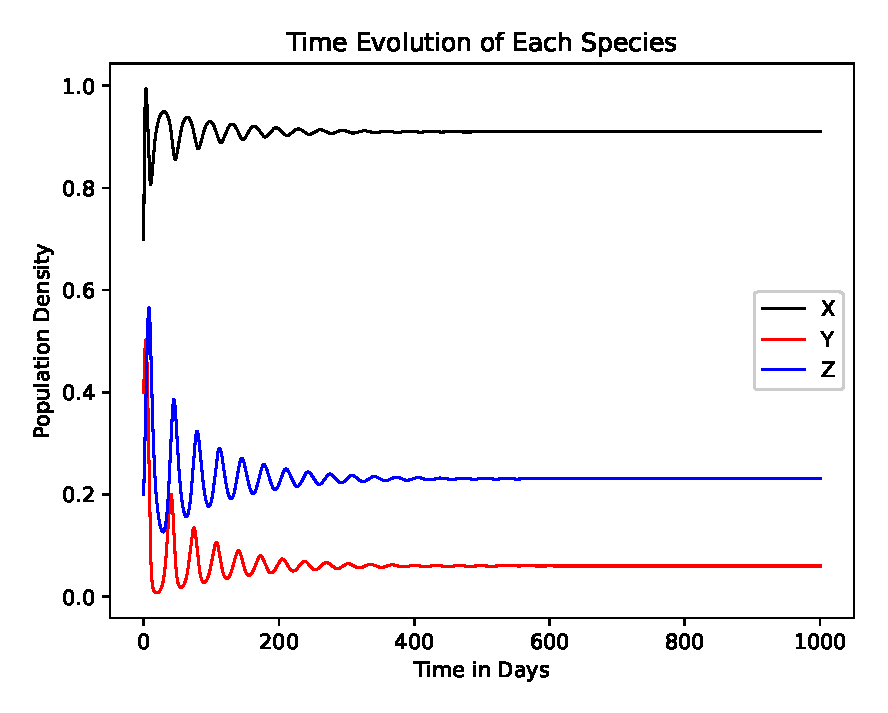
\includegraphics{equilibrium-interior-time-evolution}\label{fig:time-evolution}}}\hspace{5pt}
    \subfloat[3D phase portrait.]{%
    \resizebox*{6.88cm}{!}{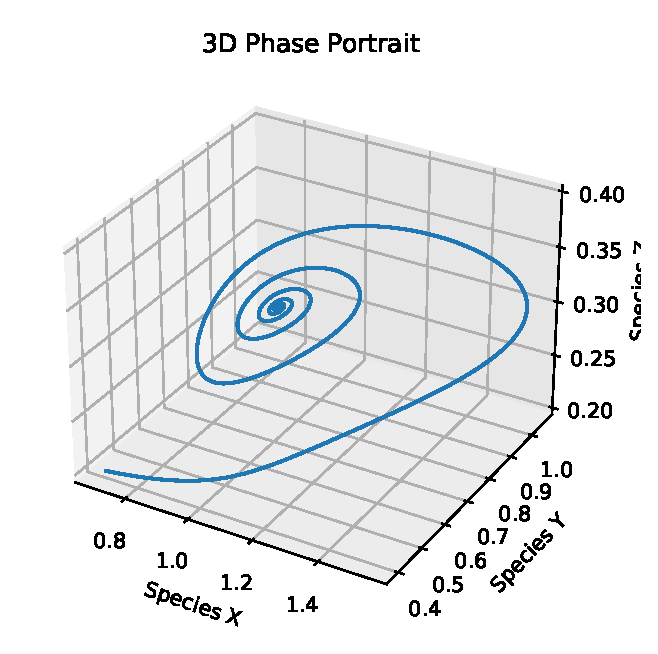
\includegraphics{equilibrium-interior-pp-xyz}\label{fig:phase-plane-3d}}}\hspace{5pt}
    \subfloat[$xy$-phase plane.]{%
    \resizebox*{6.88cm}{!}{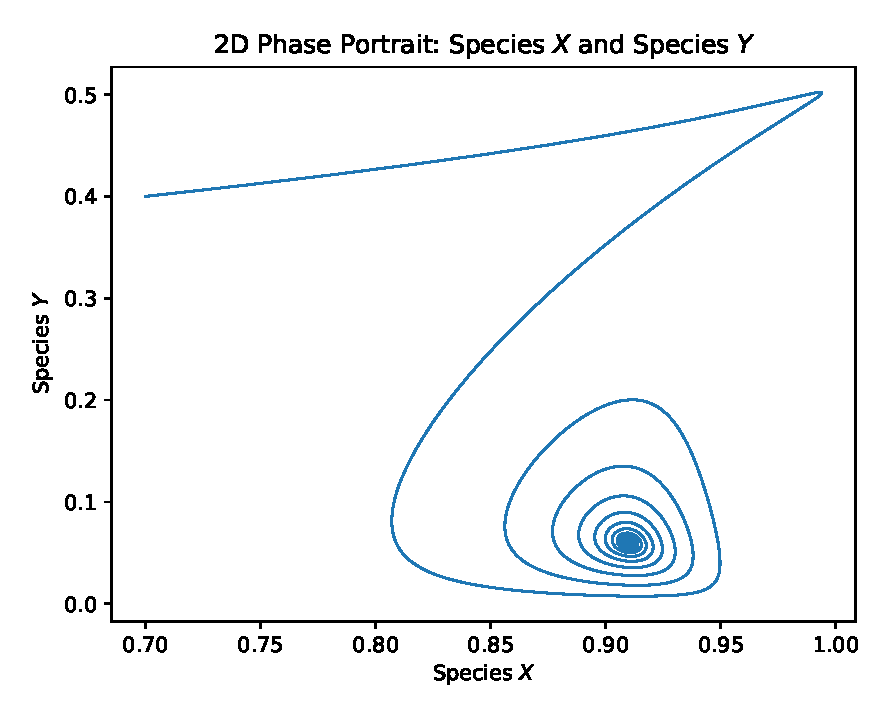
\includegraphics{equilibrium-interior-pp-xy}\label{fig:phase-plane-xy}}}\hspace{5pt}
    \subfloat[$xz$-phase plane.]{%
    \resizebox*{6.88cm}{!}{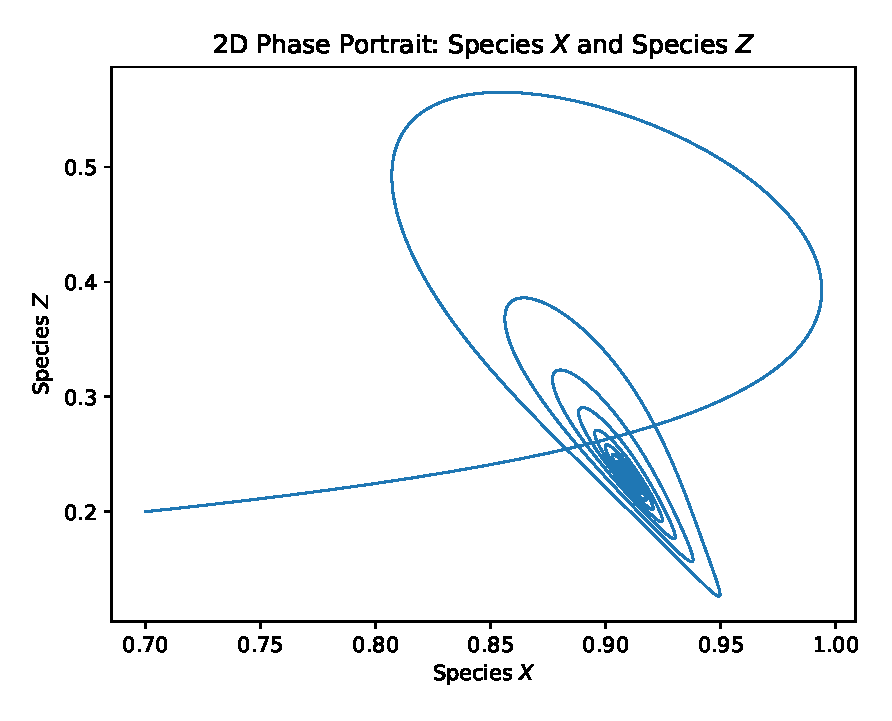
\includegraphics{equilibrium-interior-pp-xz}\label{fig:phase-plane-xz}}}\hspace{5pt}
    \subfloat[$yz$-phase plane.]{%
    \resizebox*{6.88cm}{!}{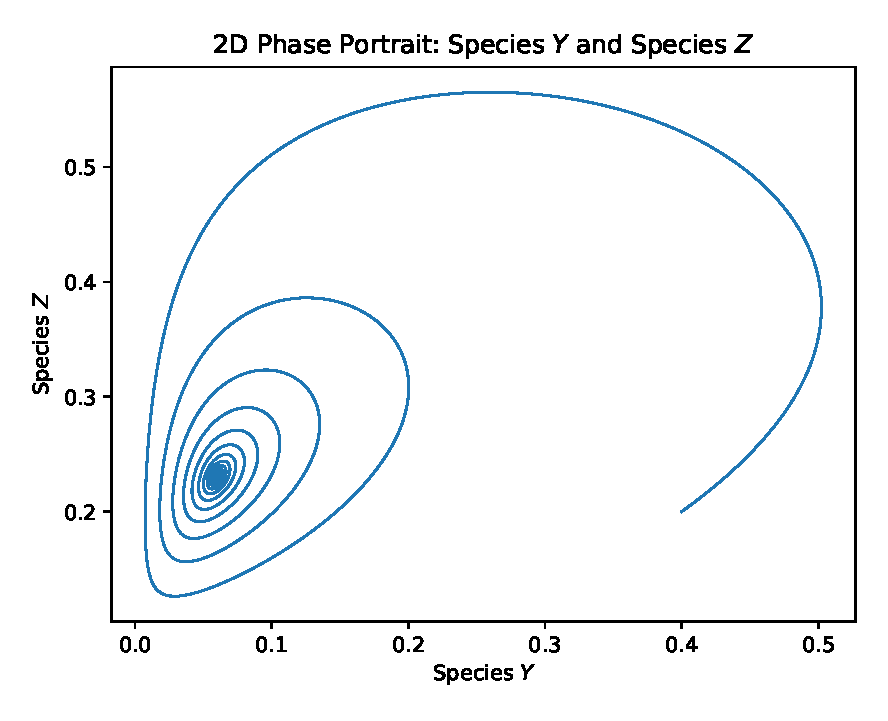
\includegraphics{equilibrium-interior-pp-yz}\label{fig:phase-plane-yz}}}
    \caption{Different types of plots to show the behavior of \myref[Model]{model:rayla-ephraim} under the set of \myref[parameters]{params:interior-a}.}
    \label{fig:nontrivial-equilibria-plots}
\end{figure}

\begin{figure}[hbt!]
    \centering
    \subfloat[Time Evolution of each species where $r_{yx}=0.5$]{%
    \resizebox*{5cm}{!}{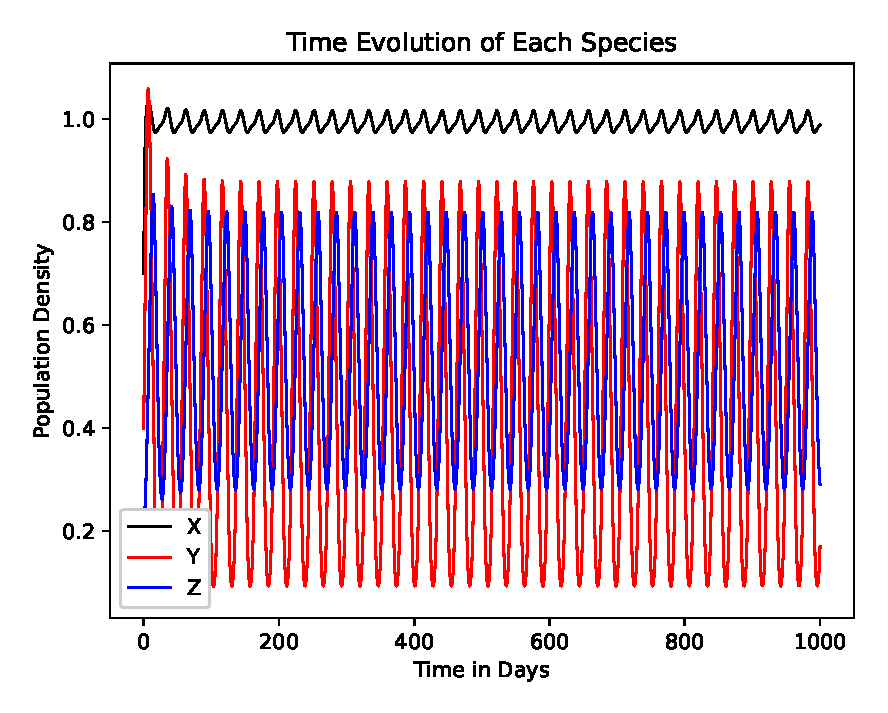
\includegraphics{equilibrium-interior-bifurcation-r_yx}\label{fig:bifurcation-r_yx-xyz}}}\hspace{5pt}
    \subfloat[Bifurcation diagram of Species $X$]{%
    \resizebox*{5cm}{!}{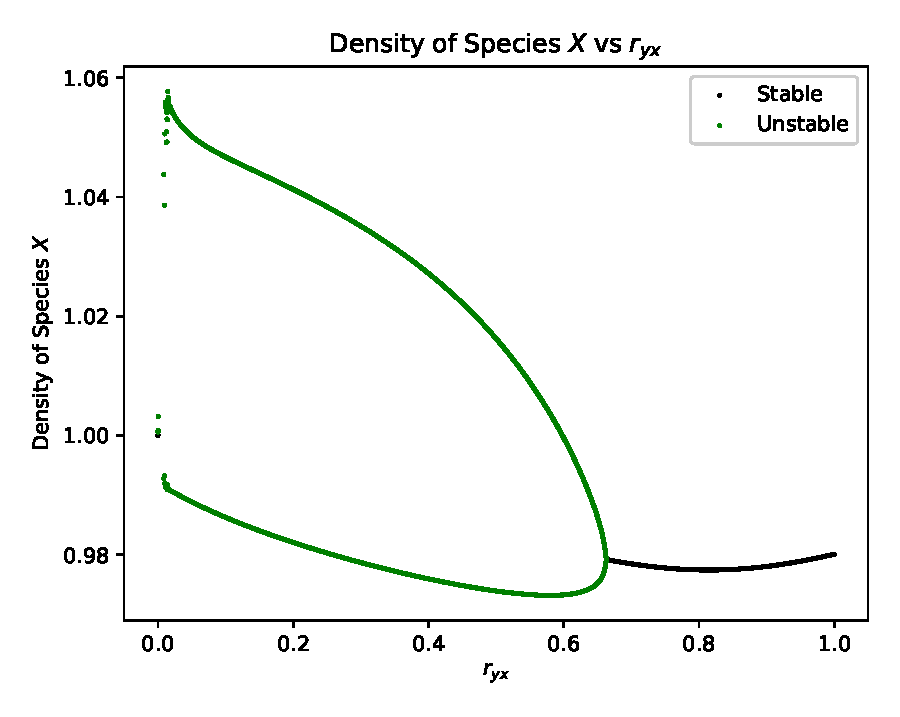
\includegraphics{equilibrium-interior-bifurcation-r_yx-x}\label{fig:bifurcation-r_yx-x}}}\hspace{5pt}
    \subfloat[Bifurcation diagram of Species $Y$]{%
    \resizebox*{5cm}{!}{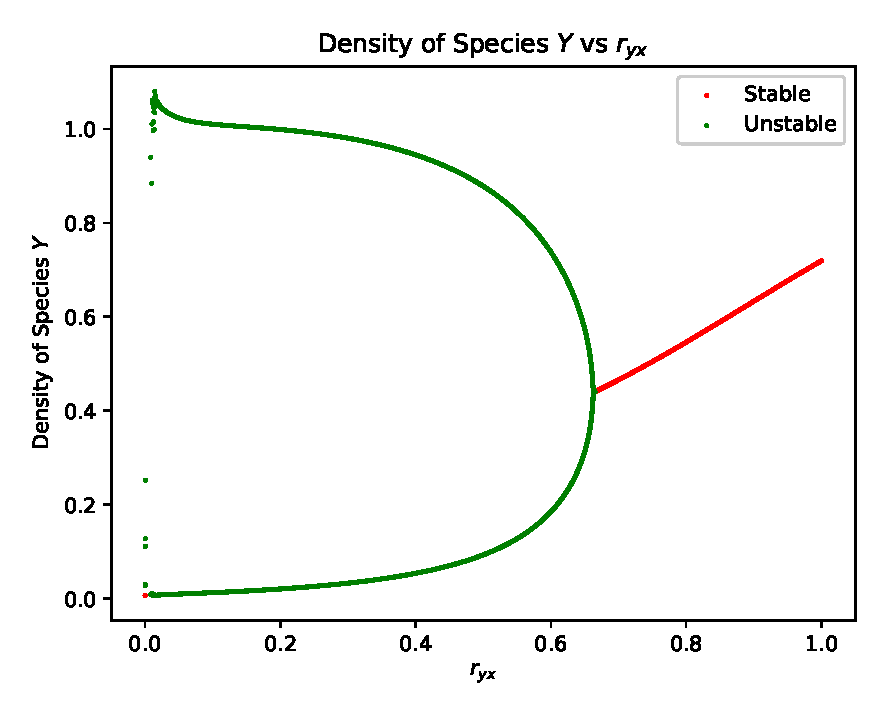
\includegraphics{equilibrium-interior-bifurcation-r_yx-y}\label{fig:bifurcation-r_yx-y}}}\hspace{5pt}
    \subfloat[Bifurcation diagram of Species $Z$]{%
    \resizebox*{5cm}{!}{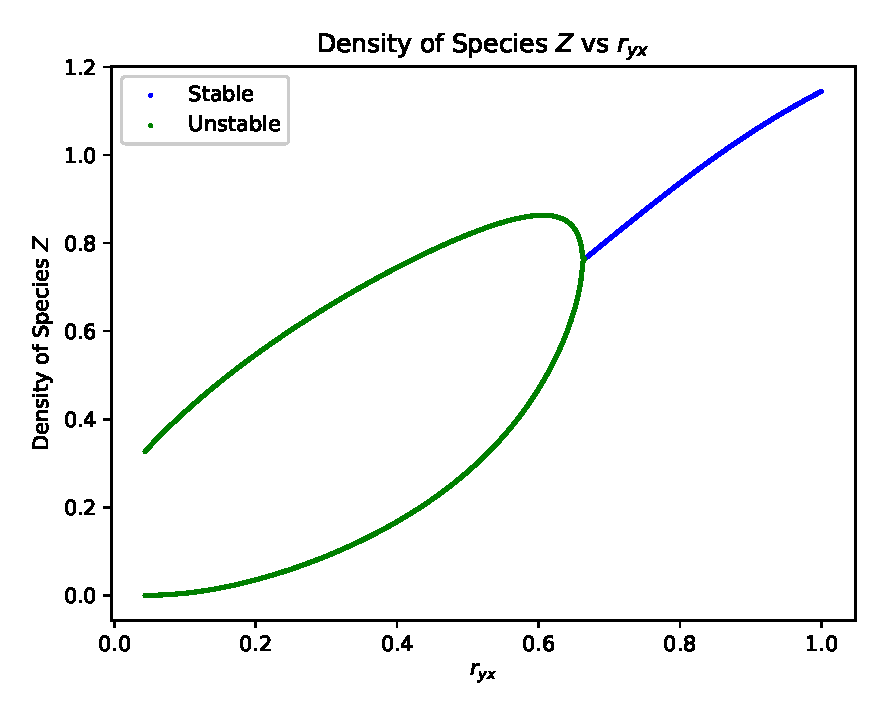
\includegraphics{equilibrium-interior-bifurcation-r_yx-z}\label{fig:bifurcation-r_yx-z}}}
    \caption{Time evolution of \myref[Model]{model:rayla-ephraim} at a specific value for $r_{yx}$ under the set of \myref[parameters]{params:interior-b} and bifurcation diagrams of each species with respect to $r_{yx}$.}
    \label{fig:bifurcation-r_yx}
\end{figure}

\begin{figure}[hbt!]
    \centering
    \subfloat[Time Evolution of each species where $r_{zx}=0.35$]{%
    \resizebox*{5cm}{!}{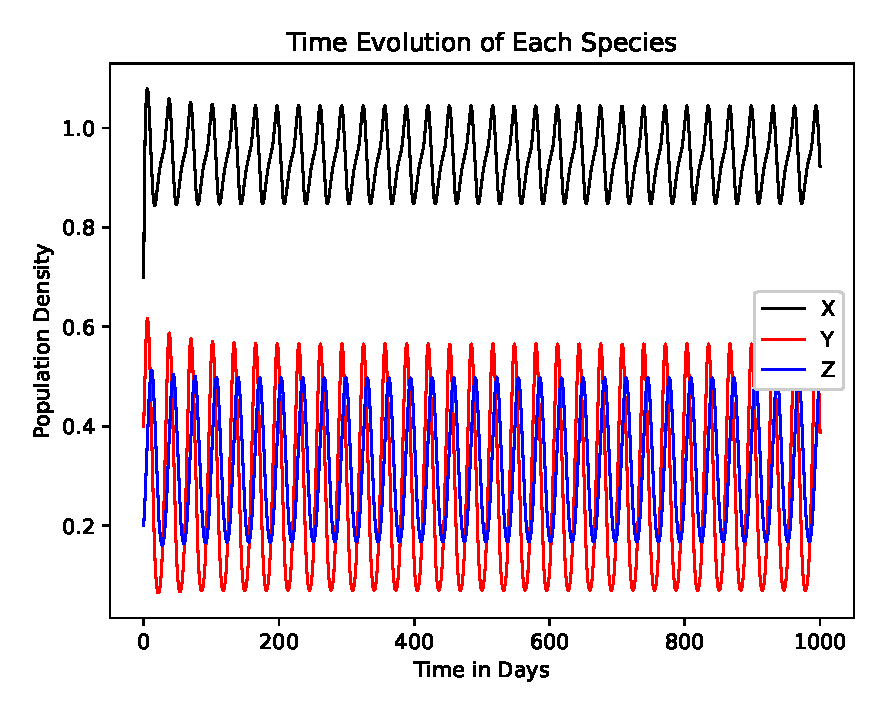
\includegraphics{equilibrium-interior-bifurcation-r_zx}\label{fig:bifurcation-r_zx-xyz}}}\hspace{5pt}
    \subfloat[Bifurcation diagram of Species $X$]{%
    \resizebox*{5cm}{!}{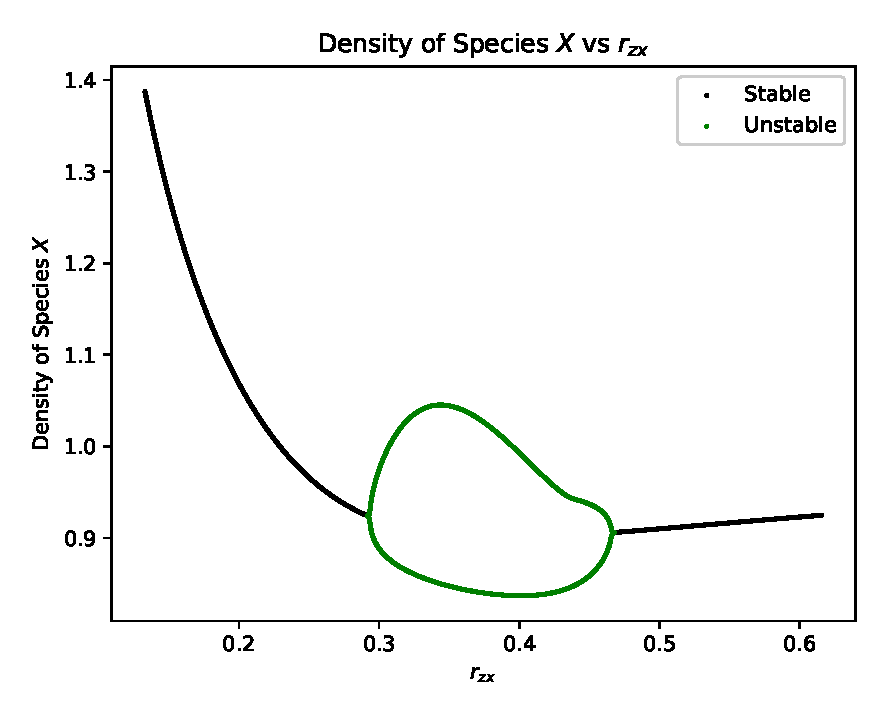
\includegraphics{equilibrium-interior-bifurcation-r_zx-x}\label{fig:bifurcation-r_zx-x}}}\hspace{5pt}
    \subfloat[Bifurcation diagram of Species $Y$]{%
    \resizebox*{5cm}{!}{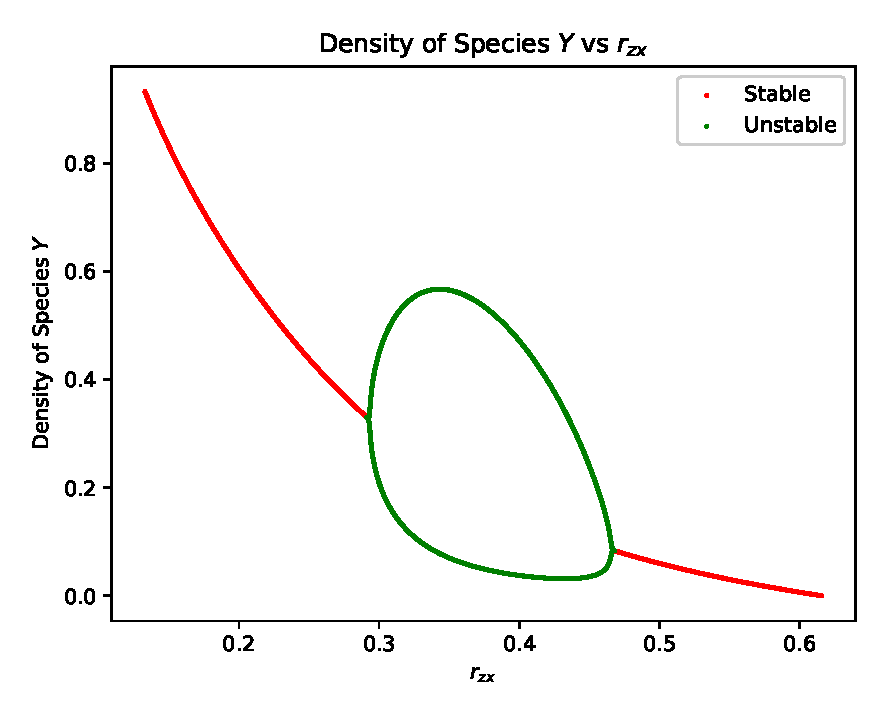
\includegraphics{equilibrium-interior-bifurcation-r_zx-y}\label{fig:bifurcation-r_zx-y}}}\hspace{5pt}
    \subfloat[Bifurcation diagram of Species $Z$]{%
    \resizebox*{5cm}{!}{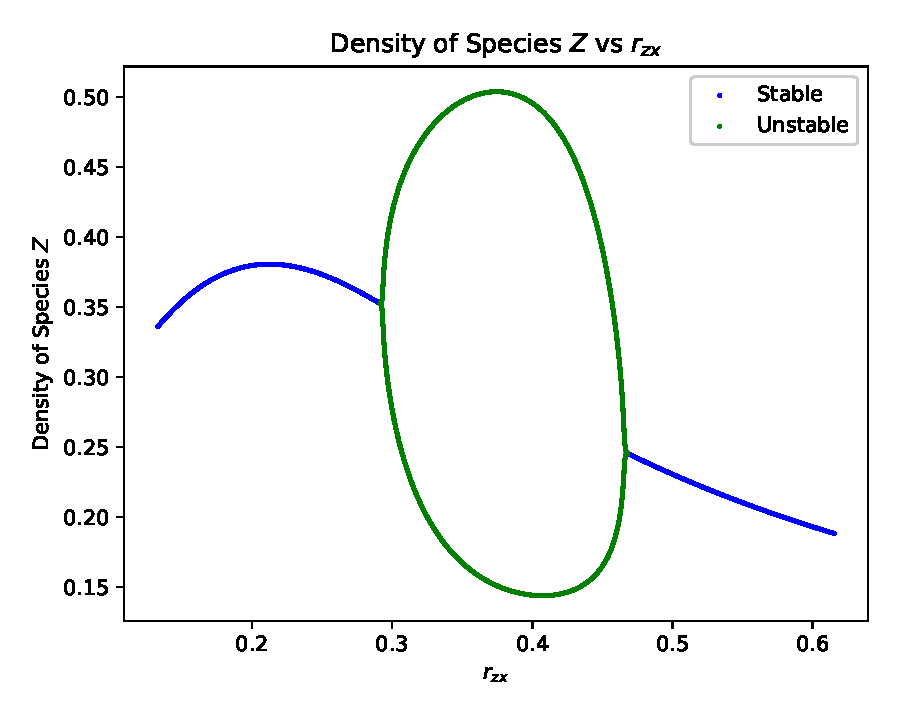
\includegraphics{equilibrium-interior-bifurcation-r_zx-z}\label{fig:bifurcation-r_zx-z}}}
    \caption{Time evolution of \myref[Model]{model:rayla-ephraim} at a specific value for $r_{zx}$ under the set of \myref[parameters]{params:interior-a} and bifurcation diagrams of each species with respect to $r_{zx}$.}
    \label{fig:bifurcation-r_zx}
\end{figure}

\begin{figure}[hbt!]
    \centering
    \subfloat[Time Evolution of each species where $p=0.1$]{%
    \resizebox*{5cm}{!}{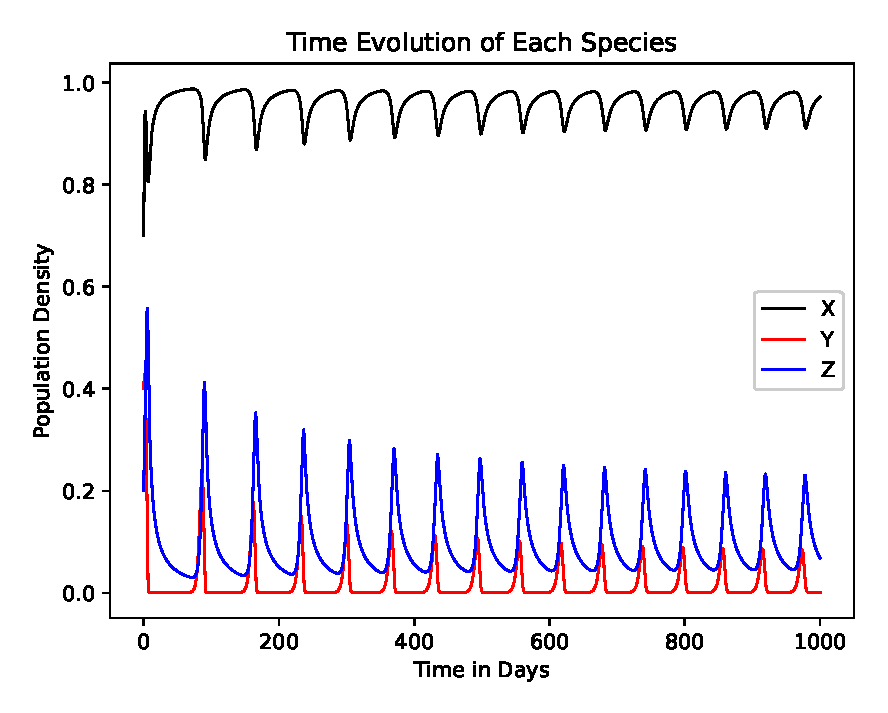
\includegraphics{equilibrium-interior-bifurcation-p}\label{fig:bifurcation-p-xyz}}}\hspace{5pt}
    \subfloat[Bifurcation diagram of Species $X$]{%
    \resizebox*{5cm}{!}{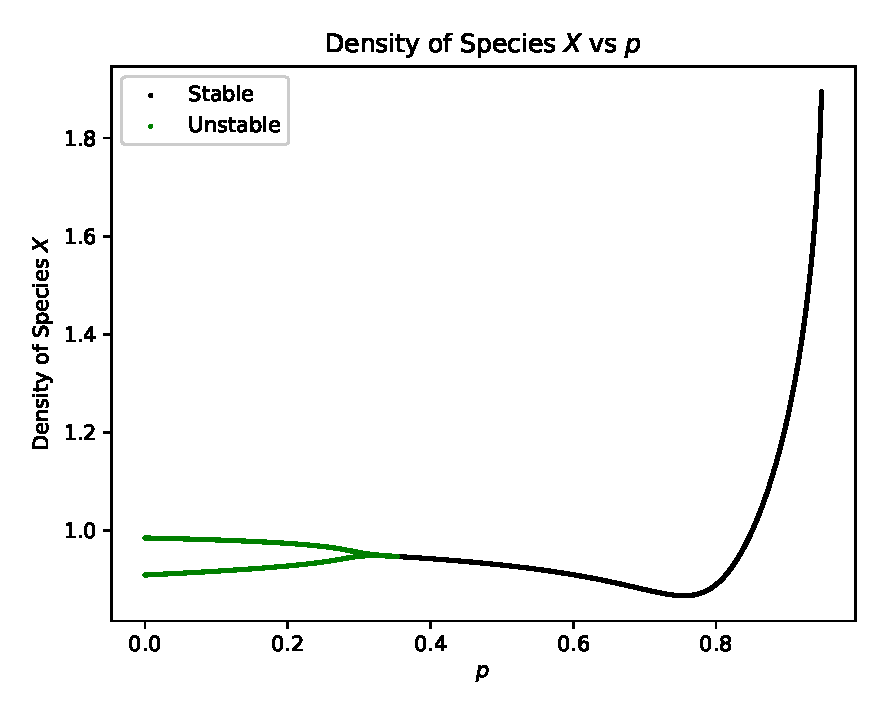
\includegraphics{equilibrium-interior-bifurcation-p-x}\label{fig:bifurcation-p-x}}}\hspace{5pt}
    \subfloat[Bifurcation diagram of Species $Y$]{%
    \resizebox*{5cm}{!}{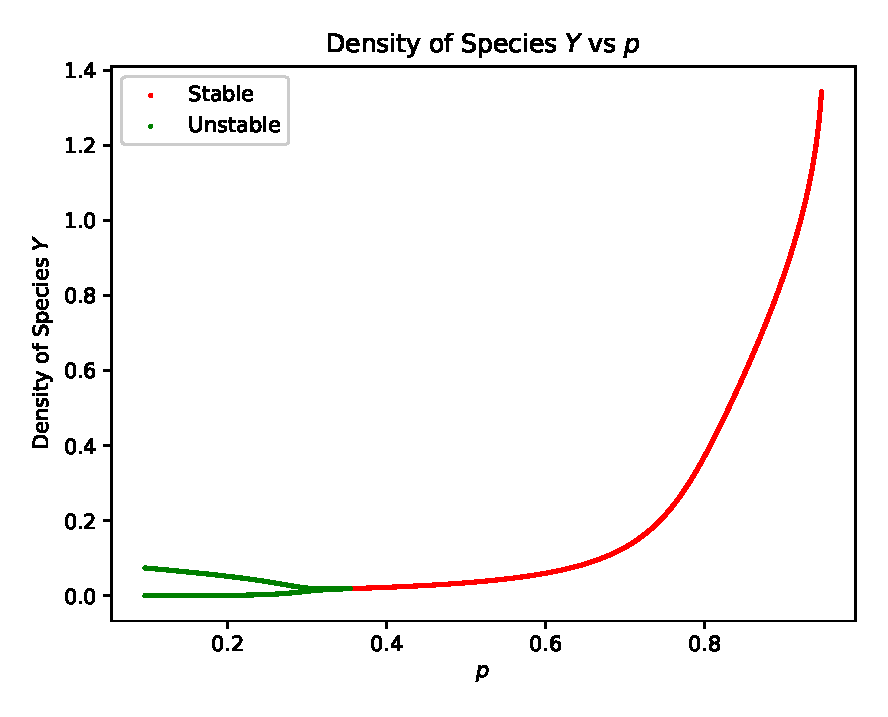
\includegraphics{equilibrium-interior-bifurcation-p-y}\label{fig:bifurcation-p-y}}}\hspace{5pt}
    \subfloat[Bifurcation diagram of Species $Z$]{%
    \resizebox*{5cm}{!}{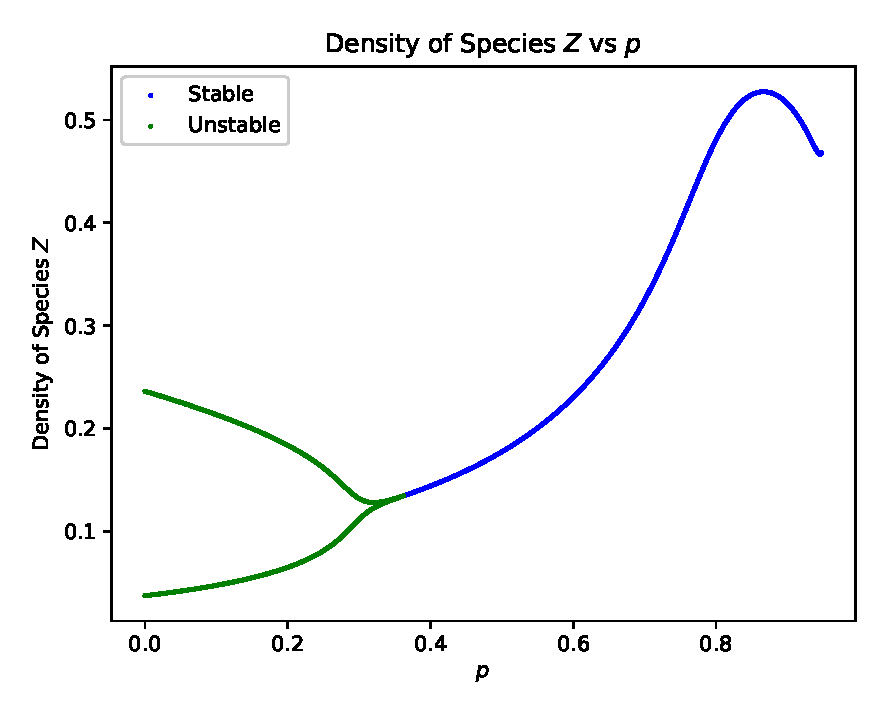
\includegraphics{equilibrium-interior-bifurcation-p-z}\label{fig:bifurcation-p-z}}}
    \caption{Time evolution of \myref[Model]{model:rayla-ephraim} at a specific value for $p$ under the set of \myref[parameters]{params:interior-a} and bifurcation diagrams of each species with respect to $p$.}
    \label{fig:bifurcation-p}
\end{figure}

\begin{figure}[hbt!]
    \centering
    \subfloat[Time Evolution of each species where $\varphi_{xy}=0.15$]{%
    \resizebox*{5cm}{!}{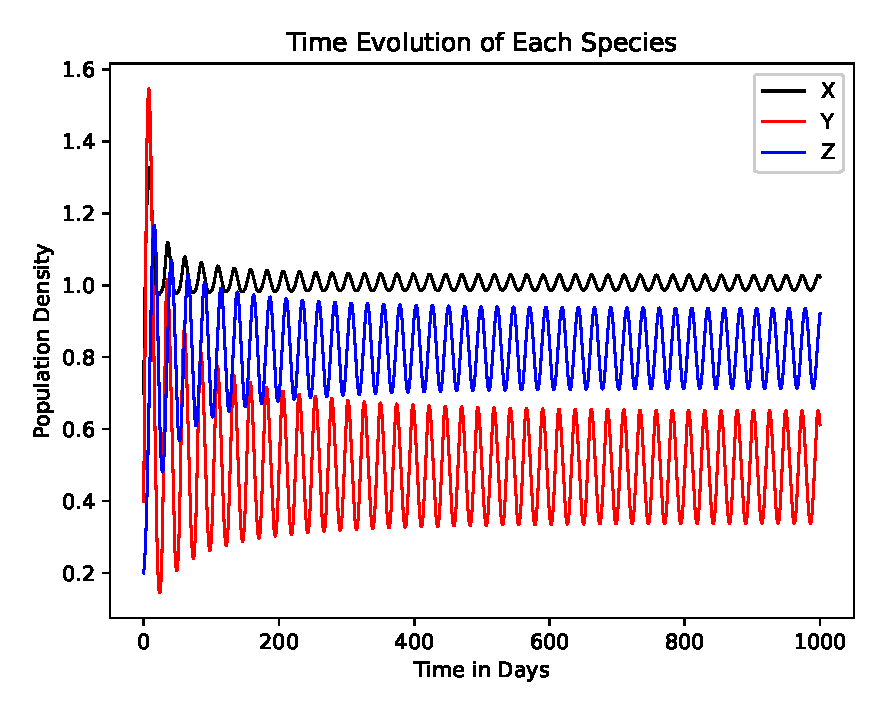
\includegraphics{equilibrium-interior-bifurcation-phi_xy}\label{fig:bifurcation-phi_xy-xyz}}}\hspace{5pt}
    \subfloat[Bifurcation diagram of Species $X$]{%
    \resizebox*{5cm}{!}{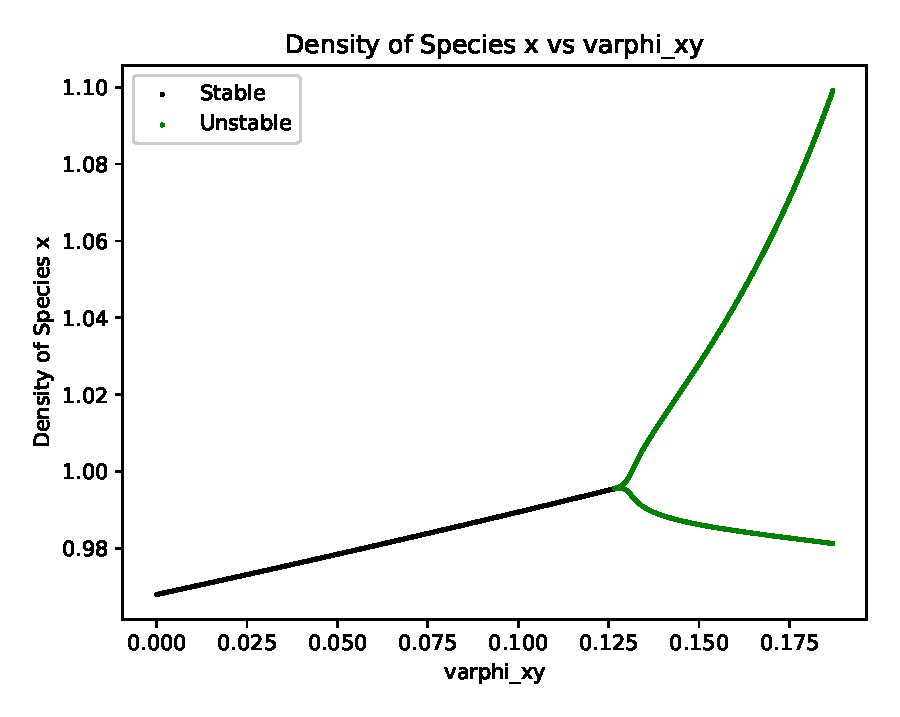
\includegraphics{equilibrium-interior-bifurcation-phi_xy-x}\label{fig:bifurcation-phi_xy-x}}}\hspace{5pt}
    \subfloat[Bifurcation diagram of Species $Y$]{%
    \resizebox*{5cm}{!}{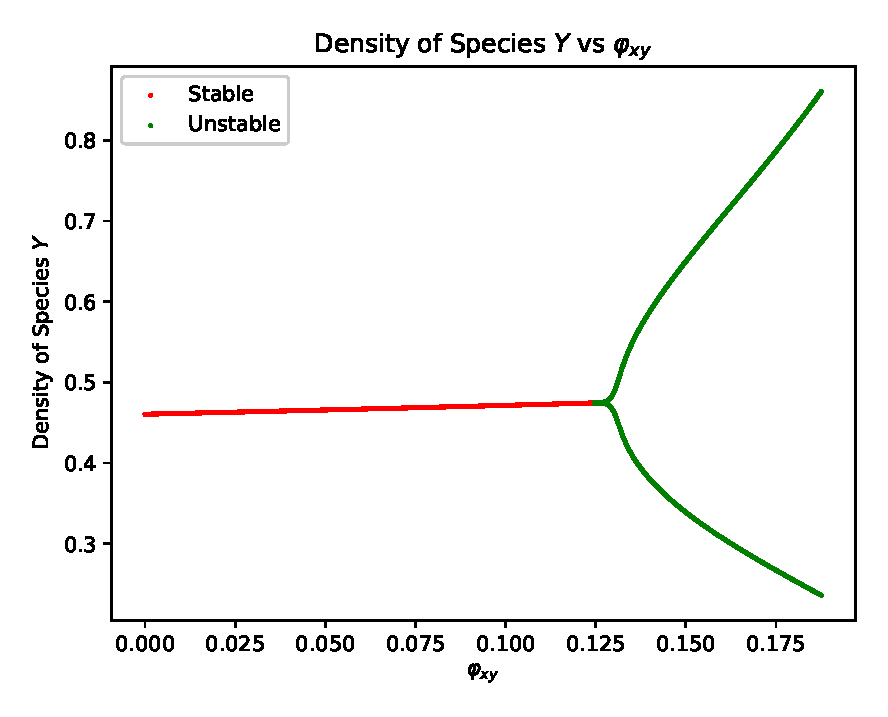
\includegraphics{equilibrium-interior-bifurcation-phi_xy-y}\label{fig:bifurcation-phi_xy-y}}}\hspace{5pt}
    \subfloat[Bifurcation diagram of Species $Z$]{%
    \resizebox*{5cm}{!}{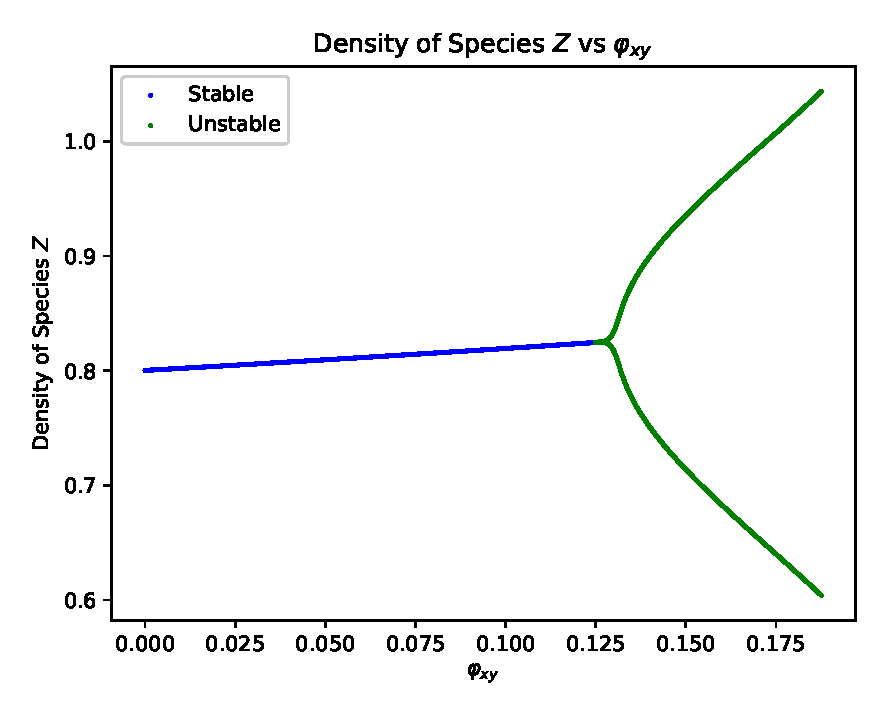
\includegraphics{equilibrium-interior-bifurcation-phi_xy-z}\label{fig:bifurcation-phi_xy-z}}}
    \caption{Time evolution of \myref[Model]{model:rayla-ephraim} at a specific value for $\varphi_{xy}$ under the set of \myref[parameters]{params:interior-b} and bifurcation diagrams of each species with respect to $\varphi_{xy}$.}
    \label{fig:bifurcation-phi_xy}
\end{figure}

\begin{figure}[hbt!]
    \centering
    \subfloat[Time Evolution of each species where $\varphi_{yx}=0.43$]{%
    \resizebox*{5cm}{!}{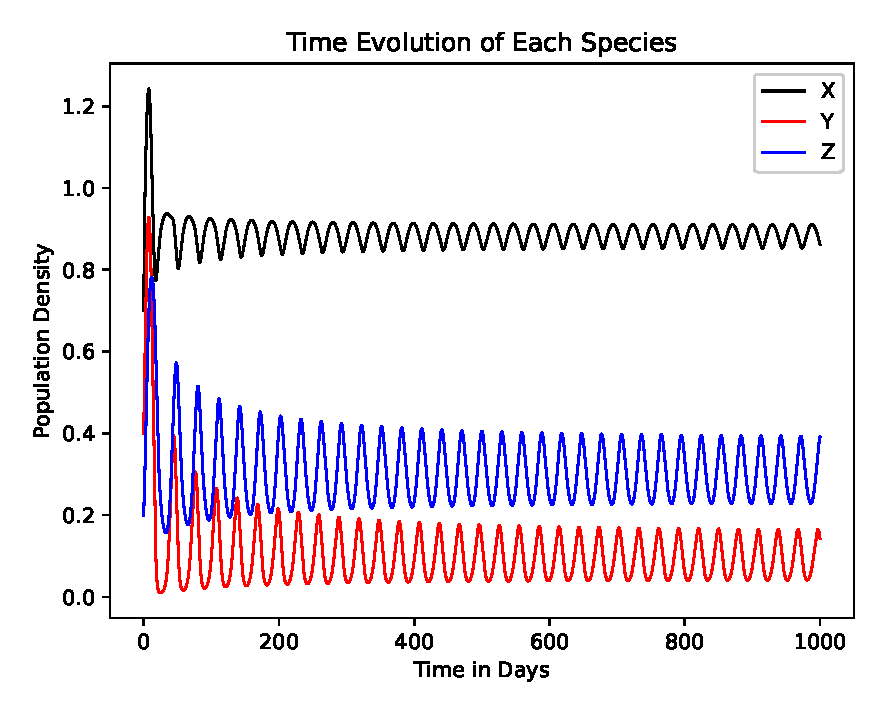
\includegraphics{equilibrium-interior-bifurcation-phi_yx}\label{fig:bifurcation-phi_yx-xyz}}}\hspace{5pt}
    \subfloat[Bifurcation diagram of Species $X$]{%
    \resizebox*{5cm}{!}{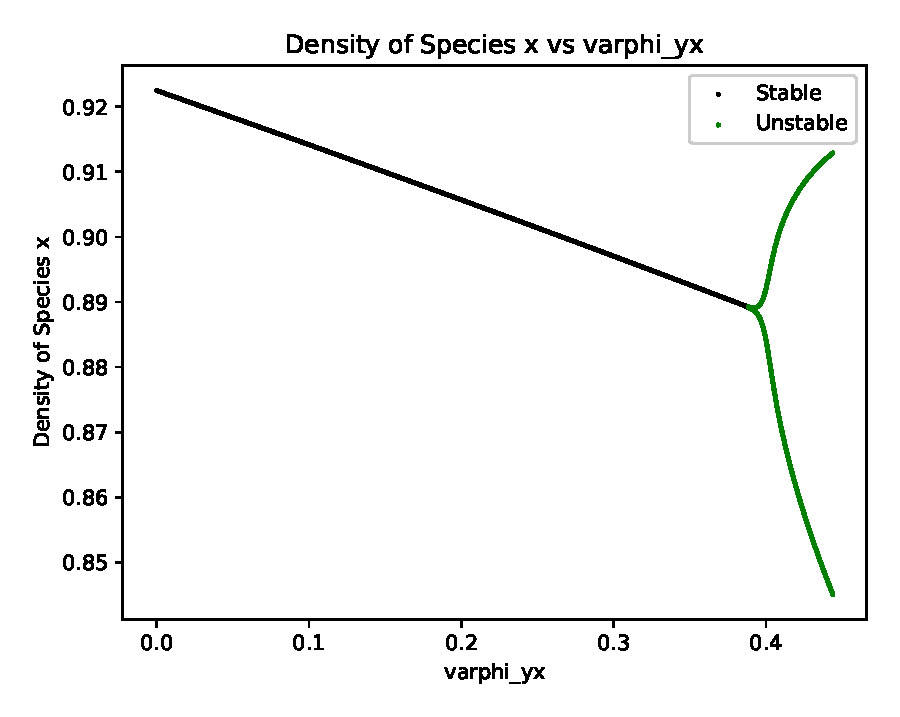
\includegraphics{equilibrium-interior-bifurcation-phi_yx-x}\label{fig:bifurcation-phi_yx-x}}}\hspace{5pt}
    \subfloat[Bifurcation diagram of Species $Y$]{%
    \resizebox*{5cm}{!}{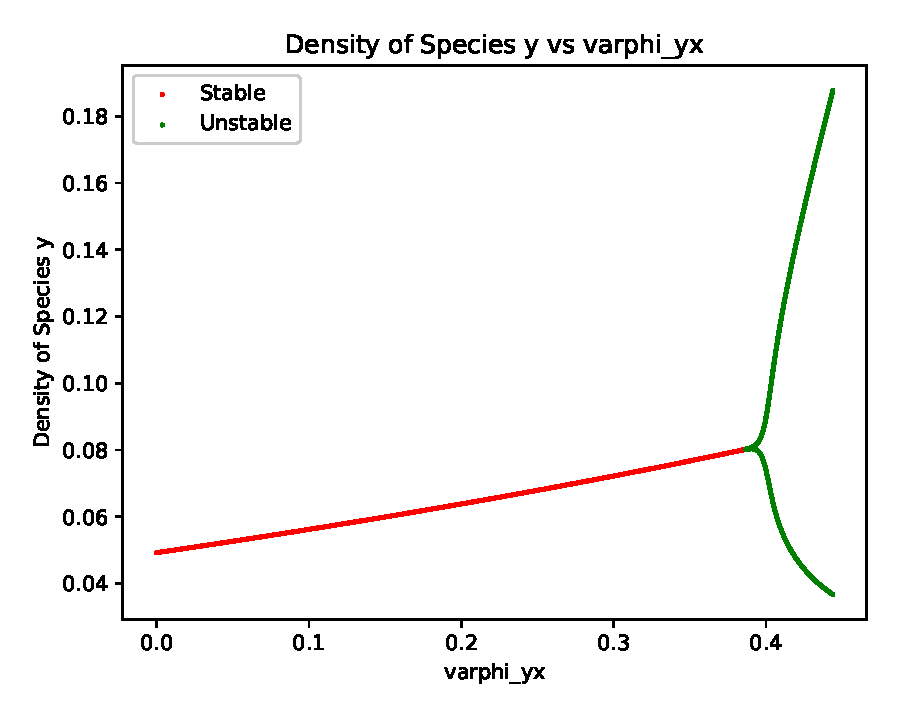
\includegraphics{equilibrium-interior-bifurcation-phi_yx-y}\label{fig:bifurcation-phi_yx-y}}}\hspace{5pt}
    \subfloat[Bifurcation diagram of Species $Z$]{%
    \resizebox*{5cm}{!}{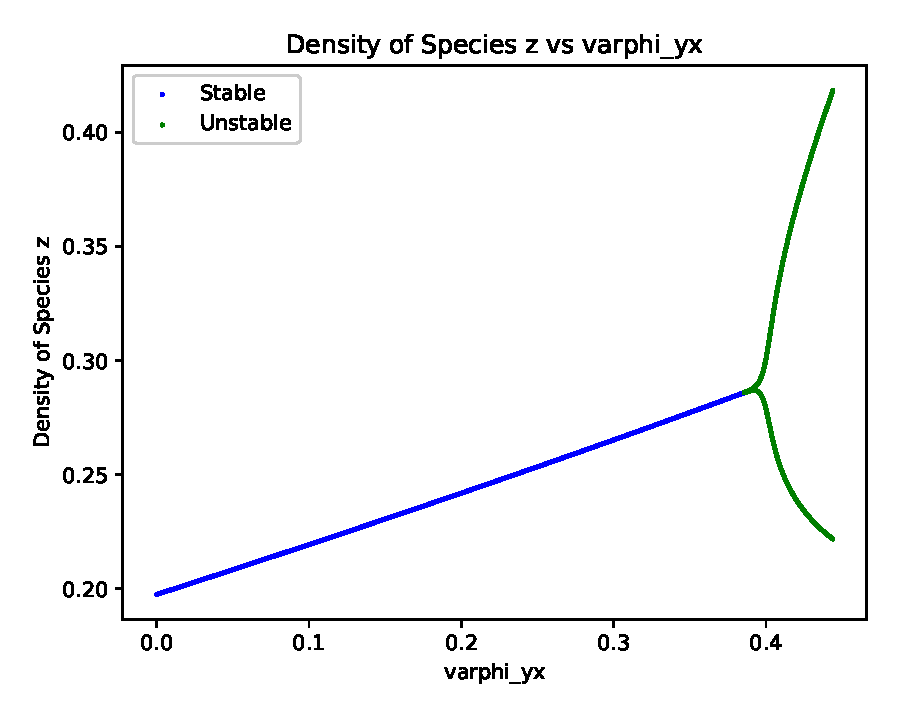
\includegraphics{equilibrium-interior-bifurcation-phi_yx-z}\label{fig:bifurcation-phi_yx-z}}}
    \caption{Time evolution of \myref[Model]{model:rayla-ephraim} at a specific value for $\varphi_{yx}$ under the set of \myref[parameters]{params:interior-a} and bifurcation diagrams of each species with respect to $\varphi_{yx}$.}
    \label{fig:bifurcation-phi_yx}
\end{figure}

\begin{figure}[hbt!]
    \centering
    \subfloat[Time Evolution of each species where $\varphi_{xz}=0.5$]{%
    \resizebox*{5cm}{!}{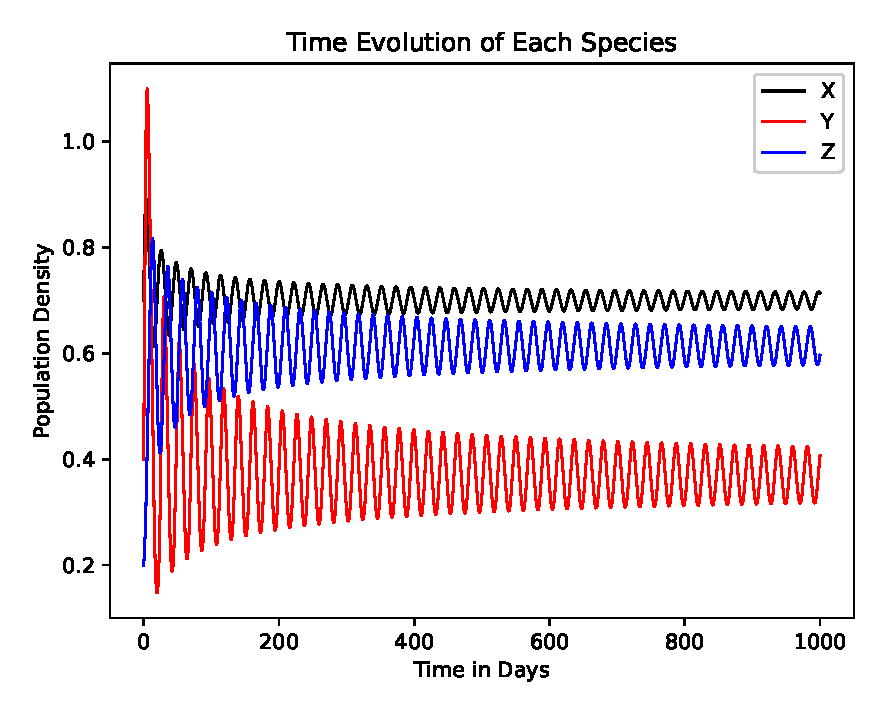
\includegraphics{equilibrium-interior-bifurcation-phi_xz}\label{fig:bifurcation-phi_xz-xyz}}}\hspace{5pt}
    \subfloat[Bifurcation diagram of Species $X$]{%
    \resizebox*{5cm}{!}{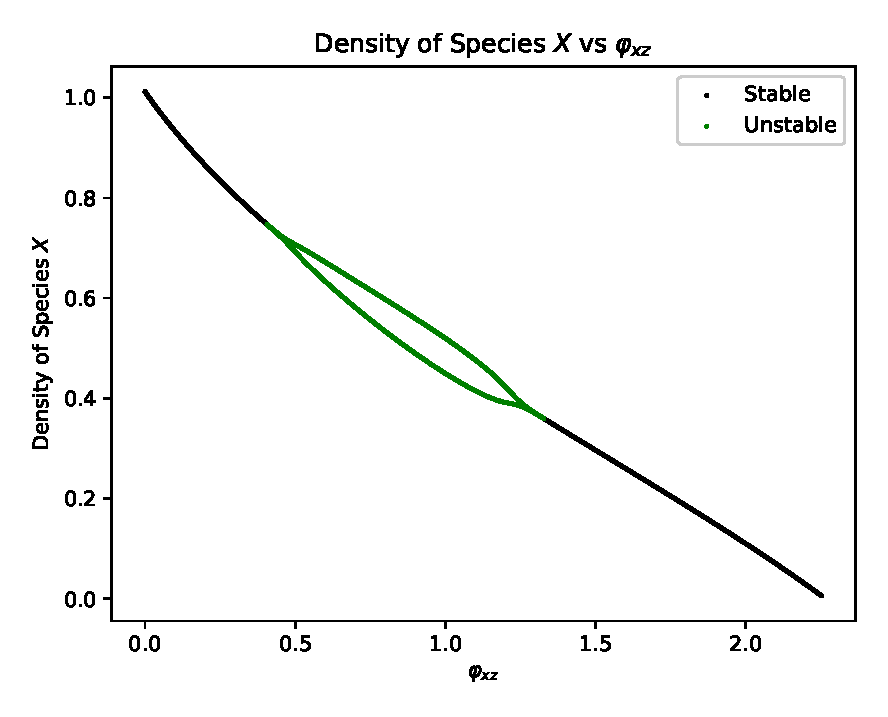
\includegraphics{equilibrium-interior-bifurcation-phi_xz-x}\label{fig:bifurcation-phi_xz-x}}}\hspace{5pt}
    \subfloat[Bifurcation diagram of Species $Y$]{%
    \resizebox*{5cm}{!}{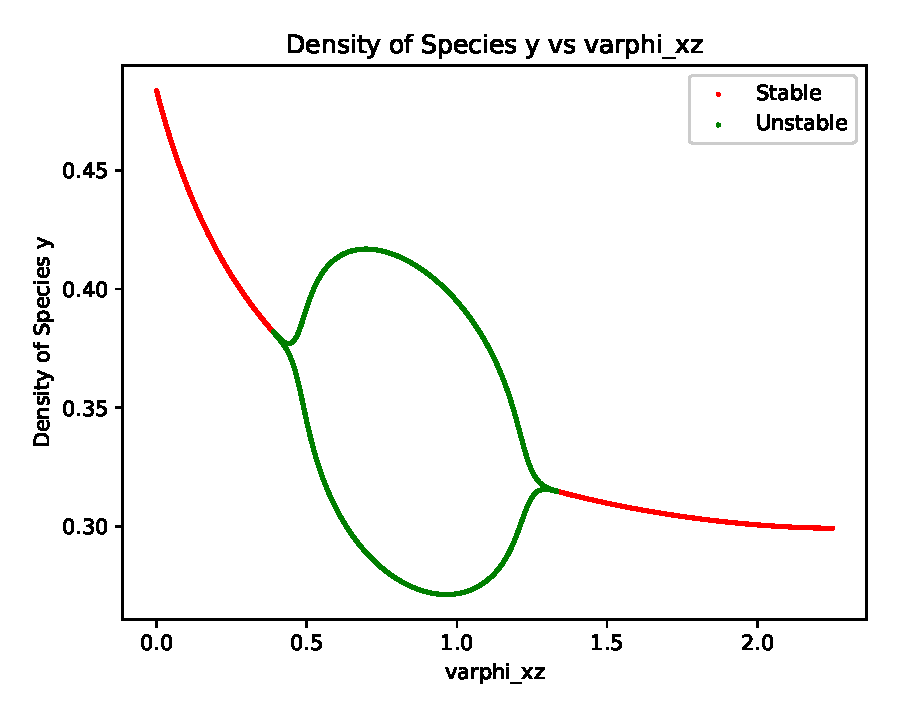
\includegraphics{equilibrium-interior-bifurcation-phi_xz-y}\label{fig:bifurcation-phi_xz-y}}}\hspace{5pt}
    \subfloat[Bifurcation diagram of Species $Z$]{%
    \resizebox*{5cm}{!}{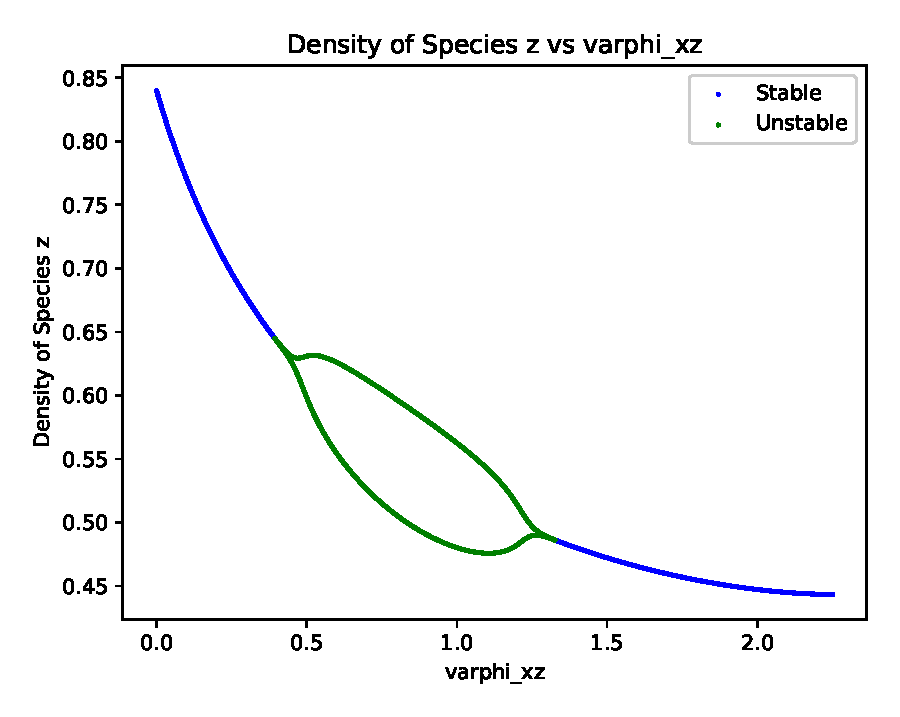
\includegraphics{equilibrium-interior-bifurcation-phi_xz-z}\label{fig:bifurcation-phi_xz-z}}}
    \caption{Time evolution of \myref[Model]{model:rayla-ephraim} at a specific value for $\varphi_{xz}$ under the set of \myref[parameters]{params:interior-b} and bifurcation diagrams of each species with respect to $\varphi_{xz}$.}
    \label{fig:bifurcation-phi_xz}
\end{figure}

\begin{figure}[hbt!]
    \centering
    \subfloat[Time Evolution of each species where $u_1=0.8$]{%
    \resizebox*{5cm}{!}{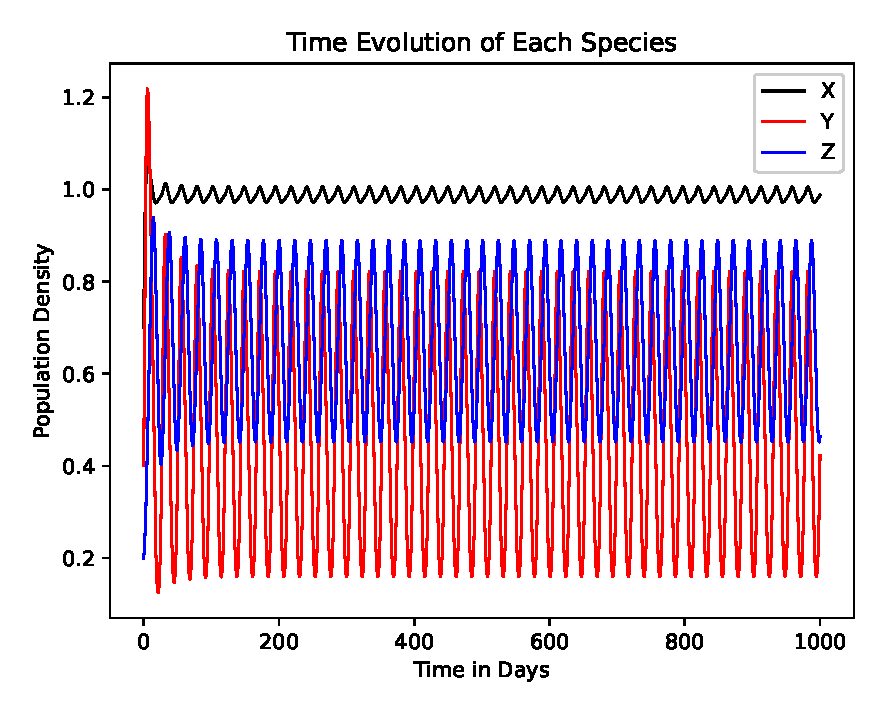
\includegraphics{equilibrium-interior-bifurcation-u_1}\label{fig:bifurcation-u_1-xyz}}}\hspace{5pt}
    \subfloat[Bifurcation diagram of Species $X$]{%
    \resizebox*{5cm}{!}{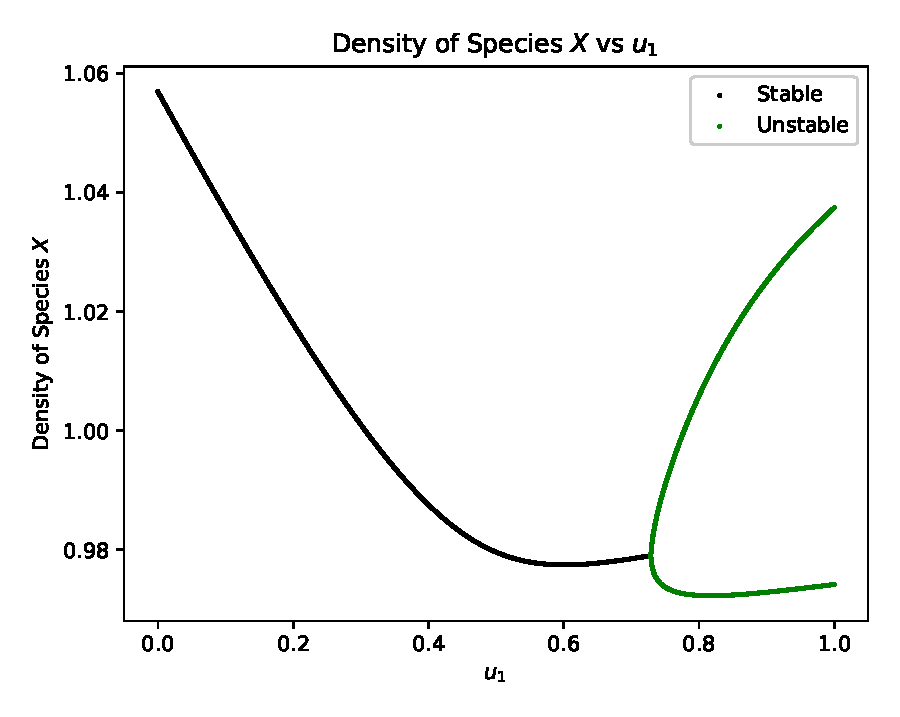
\includegraphics{equilibrium-interior-bifurcation-u_1-x}\label{fig:bifurcation-u_1-x}}}\hspace{5pt}
    \subfloat[Bifurcation diagram of Species $Y$]{%
    \resizebox*{5cm}{!}{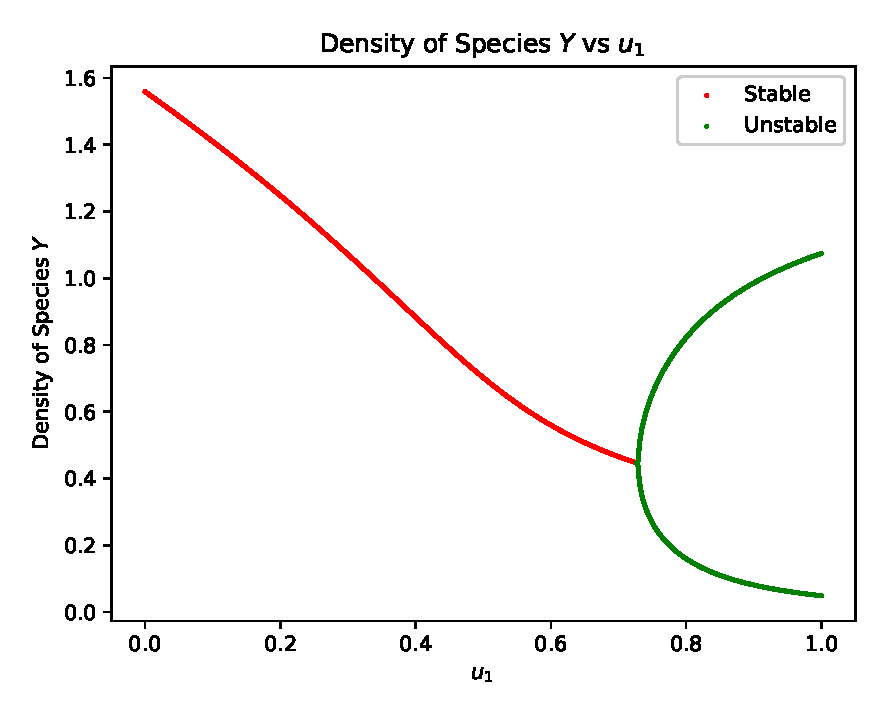
\includegraphics{equilibrium-interior-bifurcation-u_1-y}\label{fig:bifurcation-u_1-y}}}\hspace{5pt}
    \subfloat[Bifurcation diagram of Species $Z$]{%
    \resizebox*{5cm}{!}{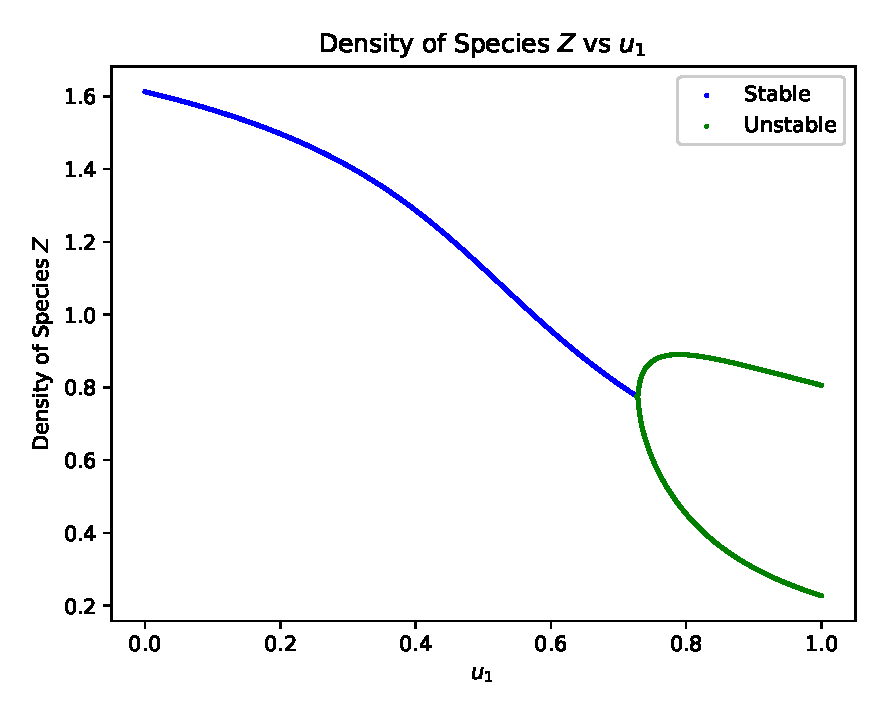
\includegraphics{equilibrium-interior-bifurcation-u_1-z}\label{fig:bifurcation-u_1-z}}}
    \caption{Time evolution of \myref[Model]{model:rayla-ephraim} at a specific value for $u_1$ under the set of \myref[parameters]{params:interior-b} and bifurcation diagrams of each species with respect to $u_1$.}
    \label{fig:bifurcation-u_1}
\end{figure}

\begin{figure}[hbt!]
    \centering
    \subfloat[Time Evolution of each species where $u_2=0.04$]{%
    \resizebox*{5cm}{!}{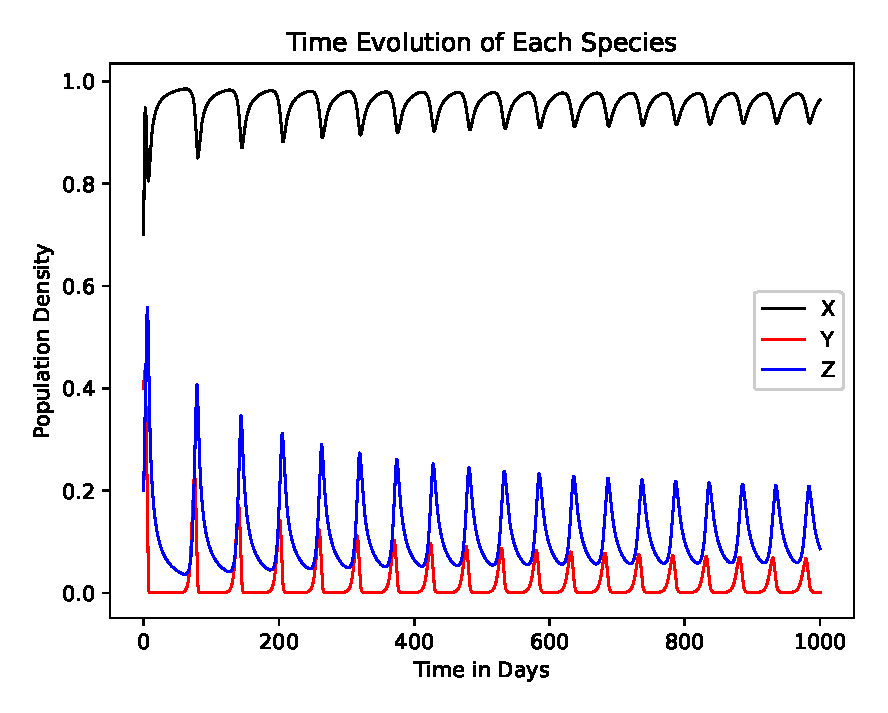
\includegraphics{equilibrium-interior-bifurcation-u_2}\label{fig:bifurcation-u_2-xyz}}}\hspace{5pt}
    \subfloat[Bifurcation diagram of Species $X$]{%
    \resizebox*{5cm}{!}{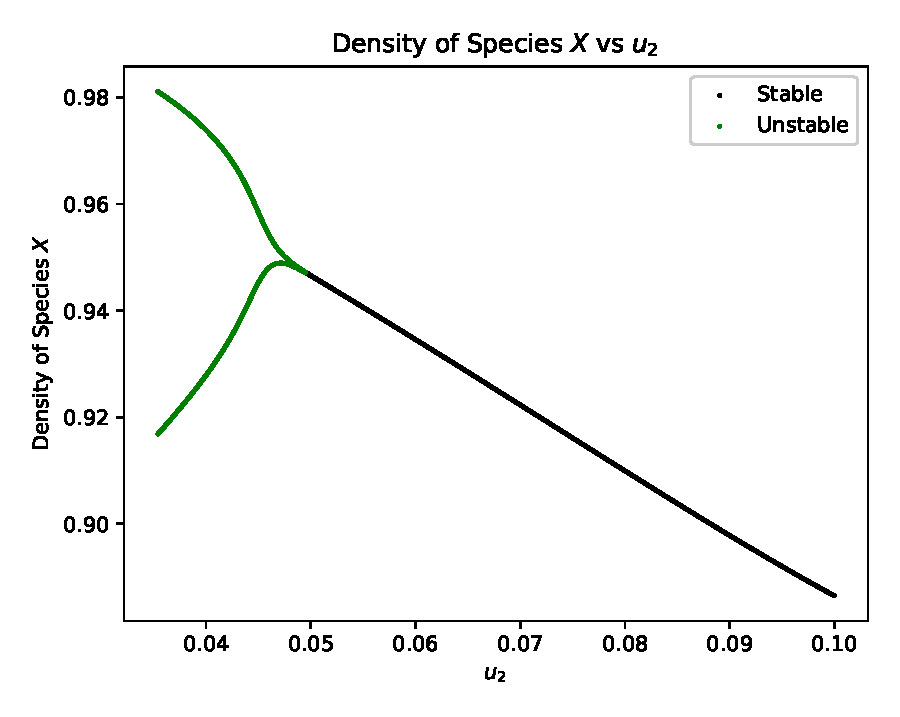
\includegraphics{equilibrium-interior-bifurcation-u_2-x}\label{fig:bifurcation-u_2-x}}}\hspace{5pt}
    \subfloat[Bifurcation diagram of Species $Y$]{%
    \resizebox*{5cm}{!}{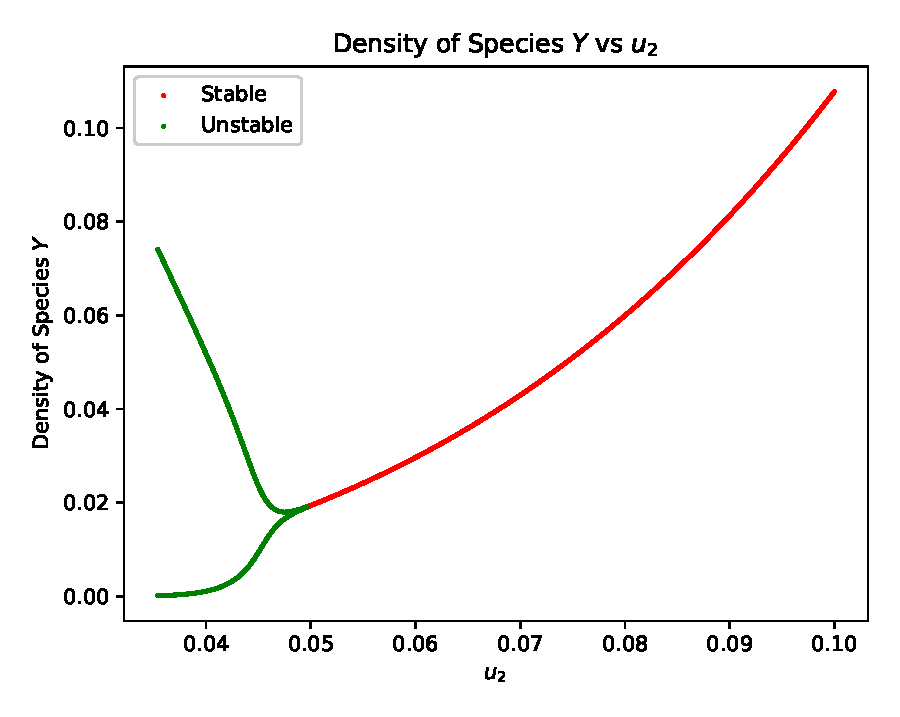
\includegraphics{equilibrium-interior-bifurcation-u_2-y}\label{fig:bifurcation-u_2-y}}}\hspace{5pt}
    \subfloat[Bifurcation diagram of Species $Z$]{%
    \resizebox*{5cm}{!}{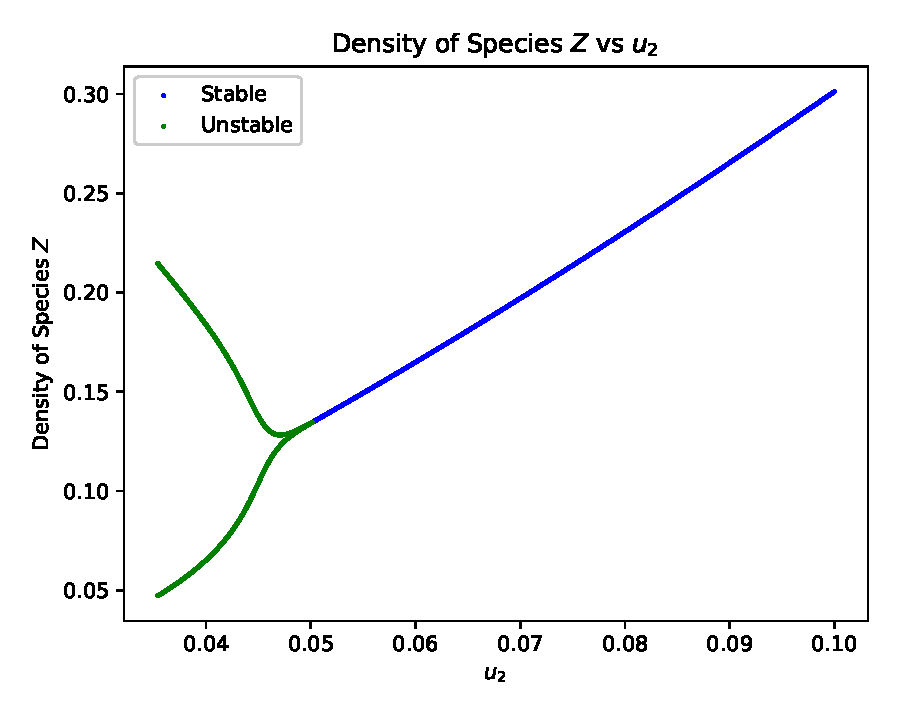
\includegraphics{equilibrium-interior-bifurcation-u_2-z}\label{fig:bifurcation-u_2-z}}}
    \caption{Time evolution of \myref[Model]{model:rayla-ephraim} at a specific value for $u_2$ under the set of \myref[parameters]{params:interior-a} and bifurcation diagrams of each species with respect to $u_2$.}
    \label{fig:bifurcation-u_2}
\end{figure}

\begin{figure}[hbt!]
    \centering
    \subfloat[Time Evolution of each species where $u_3=0.75$]{%
    \resizebox*{5cm}{!}{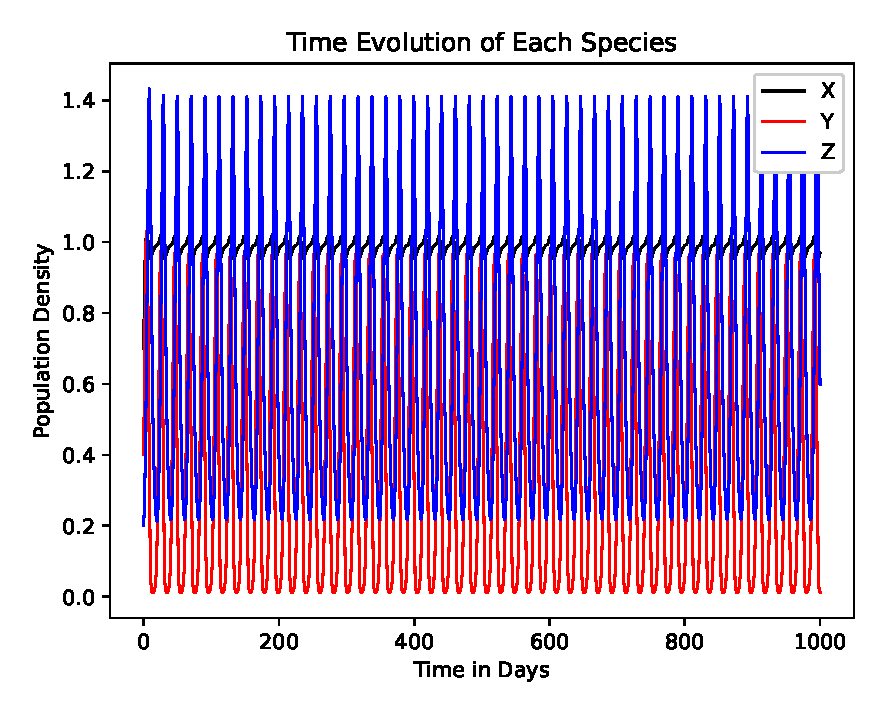
\includegraphics{equilibrium-interior-bifurcation-u_3}\label{fig:bifurcation-u_3-xyz}}}\hspace{5pt}
    \subfloat[Bifurcation diagram of Species $X$]{%
    \resizebox*{5cm}{!}{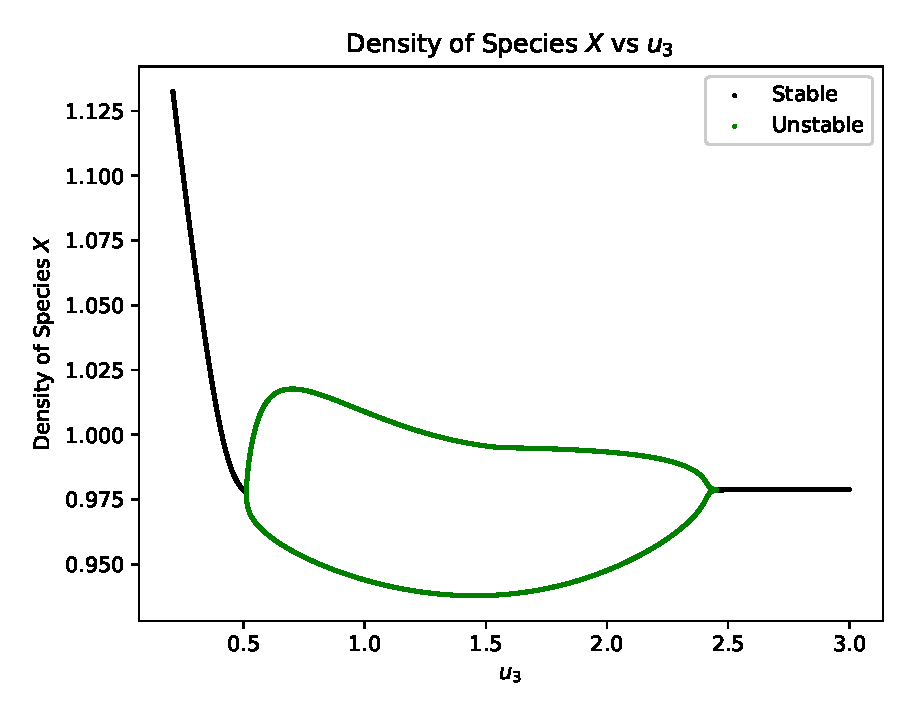
\includegraphics{equilibrium-interior-bifurcation-u_3-x}\label{fig:bifurcation-u_3-x}}}\hspace{5pt}
    \subfloat[Bifurcation diagram of Species $Y$]{%
    \resizebox*{5cm}{!}{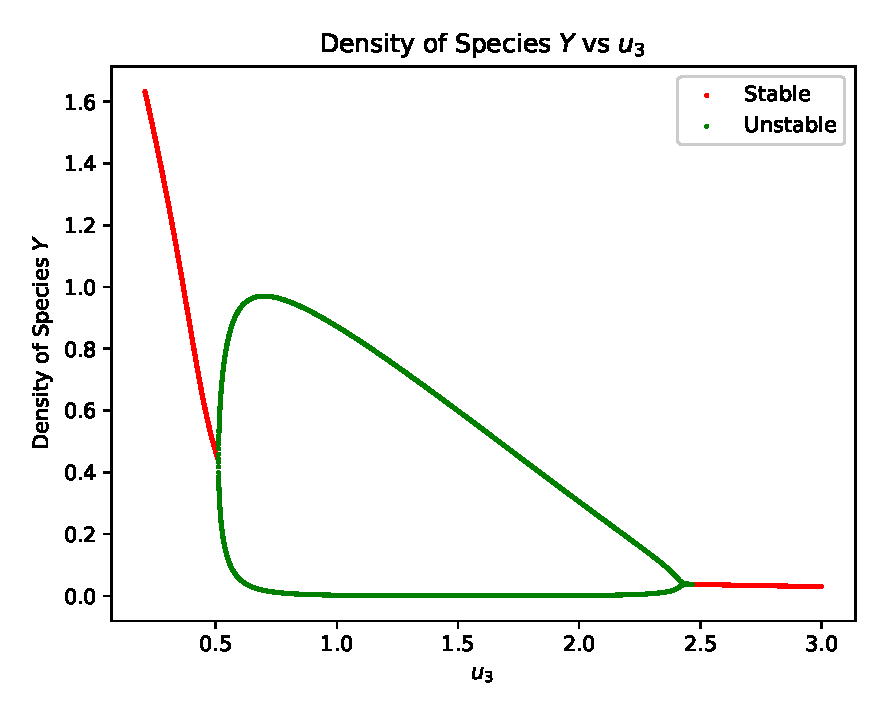
\includegraphics{equilibrium-interior-bifurcation-u_3-y}\label{fig:bifurcation-u_3-y}}}\hspace{5pt}
    \subfloat[Bifurcation diagram of Species $Z$]{%
    \resizebox*{5cm}{!}{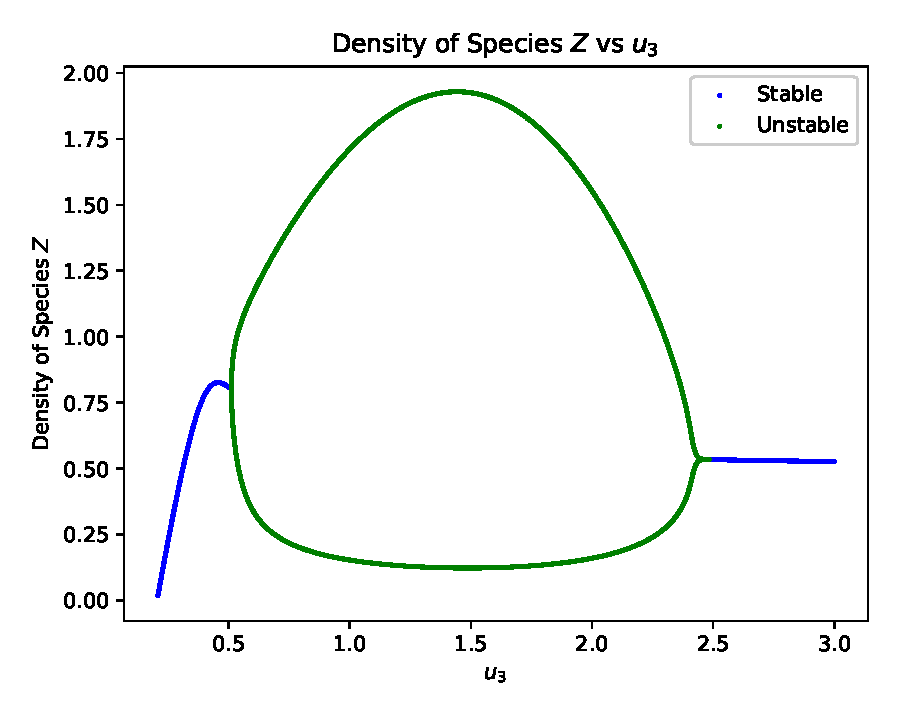
\includegraphics{equilibrium-interior-bifurcation-u_3-z}\label{fig:bifurcation-u_3-z}}}
    \caption{Time evolution of \myref[Model]{model:rayla-ephraim} at a specific value for $u_3$ under the set of \myref[parameters]{params:interior-b} and bifurcation diagrams of each species with respect to $u_3$.}
    \label{fig:bifurcation-u_3}
\end{figure}

\begin{figure}[hbt!]
    \centering
    \subfloat[Time Evolution of each species where $u_4=0.3$]{%
    \resizebox*{5cm}{!}{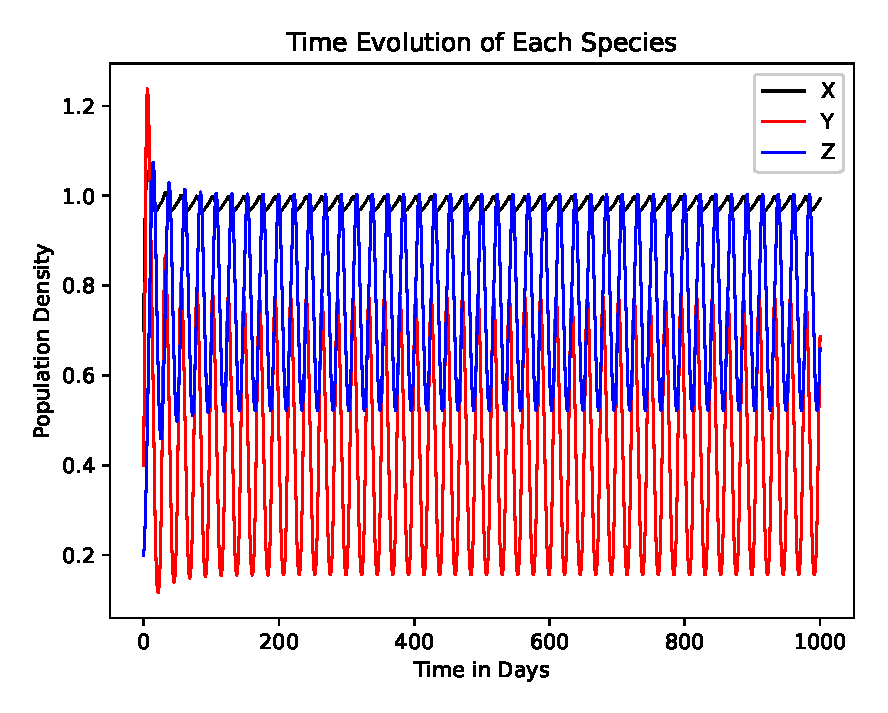
\includegraphics{equilibrium-interior-bifurcation-u_4}\label{fig:bifurcation-u_4-xyz}}}\hspace{5pt}
    \subfloat[Bifurcation diagram of Species $X$]{%
    \resizebox*{5cm}{!}{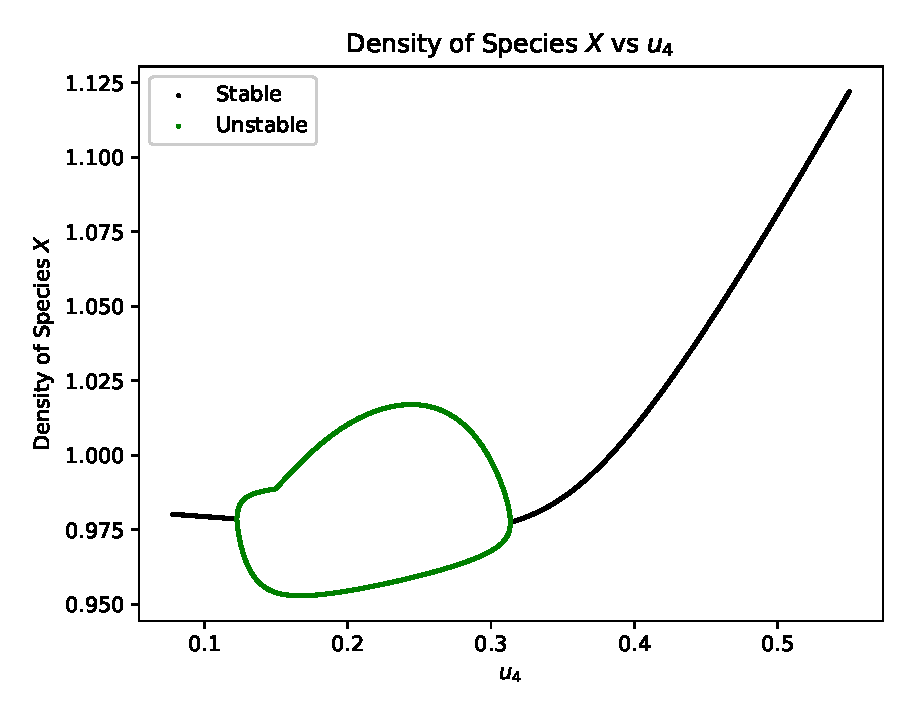
\includegraphics{equilibrium-interior-bifurcation-u_4-x}\label{fig:bifurcation-u_4-x}}}\hspace{5pt}
    \subfloat[Bifurcation diagram of Species $Y$]{%
    \resizebox*{5cm}{!}{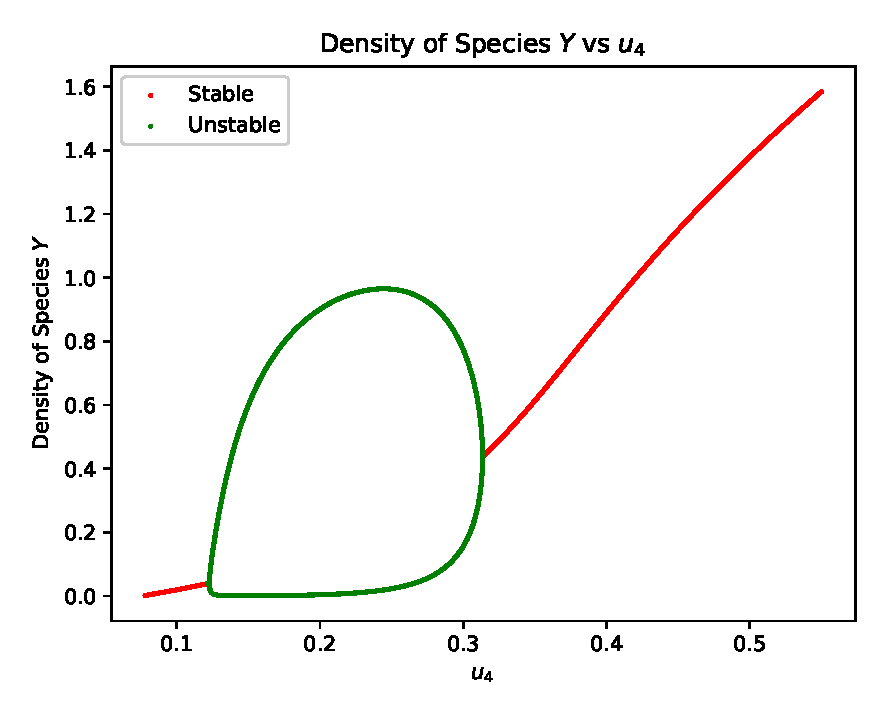
\includegraphics{equilibrium-interior-bifurcation-u_4-y}\label{fig:bifurcation-u_4-y}}}\hspace{5pt}
    \subfloat[Bifurcation diagram of Species $Z$]{%
    \resizebox*{5cm}{!}{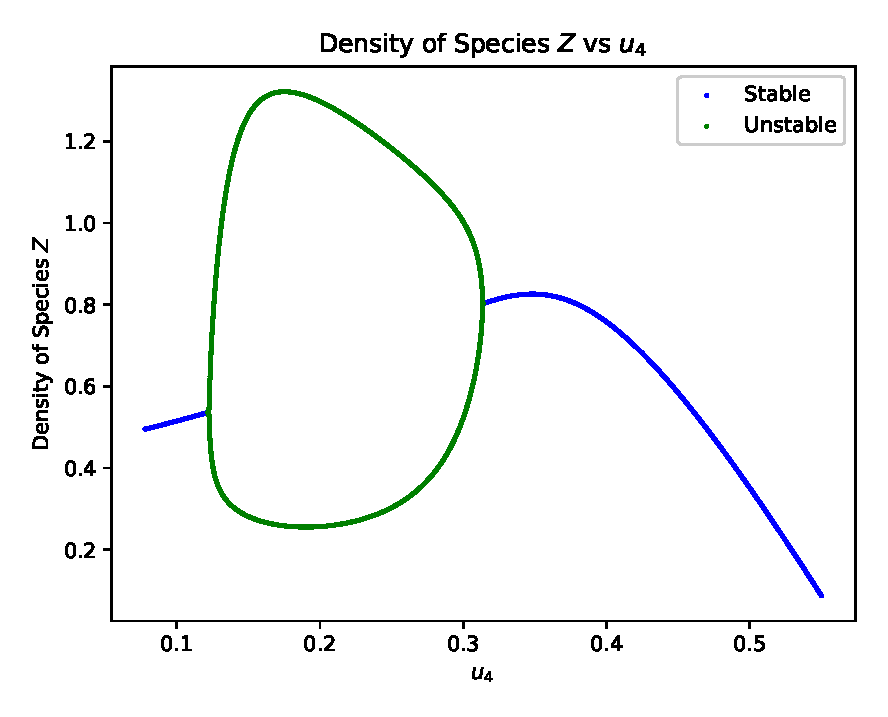
\includegraphics{equilibrium-interior-bifurcation-u_4-z}\label{fig:bifurcation-u_4-z}}}
    \caption{Time evolution of \myref[Model]{model:rayla-ephraim} at a specific value for $u_4$ under the set of \myref[parameters]{params:interior-b} and bifurcation diagrams of each species with respect to $u_4$.}
    \label{fig:bifurcation-u_4}
\end{figure}


\end{document}